\documentclass[10pt]{article}
\usepackage[french]{babel}
\usepackage[utf8]{inputenc}
\usepackage[T1]{fontenc}
\usepackage{amsmath}
\usepackage{amsfonts}
\usepackage{amssymb}
\usepackage[version=4]{mhchem}
\usepackage{stmaryrd}
\usepackage{graphicx}
\usepackage[export]{adjustbox}
\graphicspath{ {./images/} }
\usepackage{caption}
\usepackage{multirow}
\usepackage{array}
\usepackage{ragged2e}
\usepackage{enumitem}

\newcolumntype{L}[1]{>{\RaggedRight\arraybackslash}p{#1}}
\newcolumntype{C}[1]{>{\Centering\arraybackslash}p{#1}}
\newcolumntype{R}[1]{>{\RaggedLeft\arraybackslash}p{#1}}

\DeclareUnicodeCharacter{22EE}{\ifmmode\vdots\else{$\vdots$}\fi}

\begin{document}
\captionsetup{singlelinecheck=false}
\section*{Epreuve de Sciences Industrielles}
Durée 5 h

Si, au cours de l'épreuve, un candidat repère ce qui lui semble être une erreur d'énoncé, d'une part il le signale au chef de salle, d'autre part il le signale sur sa copie et poursuit sa composition en indiquant les raisons des initiatives qu'il est amené à prendre.

\section*{L'usage de calculatrices est autorisé.}
CONSIGNES :

\begin{itemize}
  \item[-] Composer lisiblement sur les copies avec un stylo à bille à encre foncée : bleue ou noire.
  \item[-] L'usage de stylo à friction, stylo plume, stylo feutre, liquide de correction et dérouleur de ruban correcteur est strictement interdit. Les surveillants et surveillantes se réservent le droit de les confisquer.
  \item[-] Remplir sur chaque copie en MAJUSCULES toutes vos informations d'identification : nom, prénom, numéro inscription, date de naissance, le libellé du concours, le libellé de l'épreuve et la session.
  \item[-] Une feuille, dont l'entête n'a pas été intégralement renseigné, ne sera pas prise en compte.
  \item[-] Il est interdit aux candidats de signer leur composition ou d'y mettre un signe quelconque pouvant indiquer sa provenance. La présence d'une information d'identification en dehors du cartouche donnera lieu à un point de pénalité et la page concernée pourra être soustraite de la correction.
\end{itemize}

Le sujet comporte les documents suivants :

\begin{itemize}
  \item[-] le texte du sujet qui comprend 25 pages
  \item[-] 5 annexes séparées
  \item[-] 3 documents réponses séparés qui seront à joindre à la copie.
\end{itemize}

Les calculatrices sont autorisées.\\
Calculatrice électronique de poche - y compris programmable, alphanumérique ou à écran graphique - à fonctionnement autonome, non imprimante, autorisée conformément à la circulaire n°99-186 du 16 novembre 1999.

Tout document et tout matériel électronique sont interdits.\\
Toute documentation autre que celle fournie est interdite.

Recommandations générales\\
L'épreuve se compose de parties indépendantes. Dans chaque partie, certaines sous-parties sont elles-mêmes indépendantes. Les candidats sont donc invités, d'une part, à lire attentivement l'énoncé avant de commencer à composer et d'autre part, à bien répartir leur temps de composition entre les différentes parties. Pour chaque partie, il est demandé aux candidats de rédiger dans l'ordre proposé par le sujet.

Il est rappelé aux candidats qu'ils doivent impérativement utiliser les notations indiquées dans le texte ou sur les figures, et qu'ils doivent présenter les calculs clairement, dégager et encadrer les résultats relatifs à chaque question référencée dans le sujet. Tout résultat incorrectement exprimé ne sera pas pris en compte. Les candidats traceront tous les schémas ou chronogrammes qui leur permettront d'étayer leurs raisonnements.

\section*{L'INJECTION PLASTIQUE}
\section*{PARTIE 1. INTRODUCTION}
\subsection*{1.1. Contexte général}
Le plastique est aujourd'hui partout autour de nous. Inventé à la fin du XIX ${ }^{\mathrm{e}}$ siècle, avec une production mondiale de 1,5 million de tonnes en 1950, la production atteignait 390 millions de tonnes en 2021. Le plastique présente de nombreux avantages : il est léger, a de bonnes caractéristiques mécaniques, présente un coût de production relativement faible, mais ce qui l'a rendu très populaire, c'est sa capacité à prendre différentes formes au gré de nos envies. Souple, rigide, transparent, opaque, étirable, durable, avec des couleurs... Tout est possible ou presque.

Le problème est que les plastiques ont des impacts très importants pour l'environnement. Ils polluent les sols et les océans, soit par pollution directe avec des déchets plastiques non mis en point de collecte, soit par pollution invisible de microplastiques issus de leur utilisation. En particulier dans les océans, on estime à un million d'oiseaux et plus de cent mille mammifères marins victimes des déchets plastiques ou microplastiques par an.

Malgré sa robustesse et sa durée de vie, il est souvent jeté trop vite. Les exemples sont nombreux, en particulier sur les plastiques à usage unique. De nombreuses interdictions ont vu le jour pour limiter ce gaspillage : en 2017, les sacs plastiques jetables ; en 2021, les produits en plastique jetables comme les couverts, les assiettes et les gobelets...etc.

En 2025 apparaissent les plastiques biosourcés qui doivent être composés d'au moins 60\% d'origine végétale. Le reste est souvent composé de produits issus de dérivés du pétrole. Ces plastiques ne sont pas forcément la solution puisqu'ils ne sont pas forcément biodégradables.

Le recyclage est donc un enjeu important pour limiter l'impact environnemental et sanitaire. Pour le moment, les matières premières vierges issues du pétrole sont encore moins chères que les matières recyclées. En cause, le tri des différents plastiques mais aussi les composés font appel à des particules ou fibres non plastiques dont la séparation est complexe.

\subsection*{1.2. Procédé de fabrication d'objet plastique}
A partir de matière première vierge ou recyclée, les procédés de fabrication d'objets en plastique sont divers :

\begin{itemize}
  \item[-] Impression 3D ou dite fabrication additive : elle consiste à déposer couche par couche la matière plastique pour former la pièce finale.
  \item[-] Moulage par extrusion : la matière plastique chauffée est extrudée par un orifice ayant la forme de la pièce désirée, elle permet de produire des pièces linéiques à forme constante comme des tubes, feuilles ou profilés.
  \item[-] Moulage par compression : la matière chaude est déposée dans un moule puis maintenue à la forme désirée par compression pendant une phase de refroidissement et de durcissement.
  \item[-] Moulage par soufflage : elle est utilisée pour produire des pièces creuses comme des bouteilles, bidons... On injecte de l'air comprimé soufflé à l'intérieur de la matière préformée, permettant à la matière de se dilater et d'épouser la forme interne du moule.
  \item[-] Moulage par injection : c'est la méthode la plus utilisée. La matière plastique chauffée est injectée dans un moule, prenant la forme de la pièce souhaitée.
\end{itemize}

\subsection*{1.3. Injection plastique}
\begin{figure}[h]
\begin{center}
  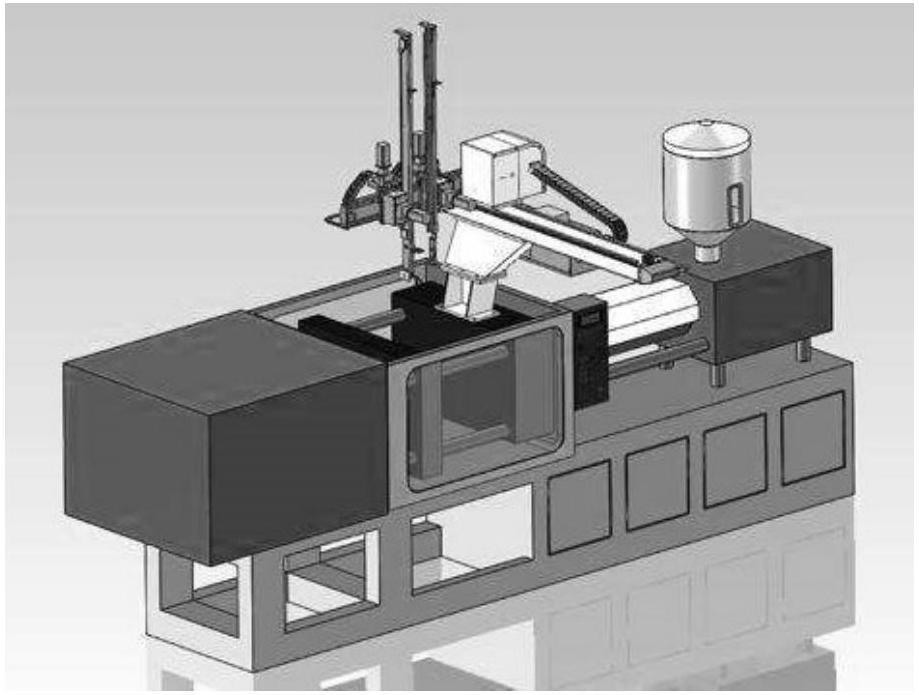
\includegraphics[alt={},max width=\textwidth]{076c1ba0-5a37-41d5-876a-83fc91dd5c32-04_695_919_342_574}
\captionsetup{labelformat=empty}
\caption{Figure 1 : Vue d'ensemble d'une machine à injection plastique}
\end{center}
\end{figure}

La quasi-totalité des machines à injection plastique ont la même architecture, une représentation est donnée figure 2. Elle se compose d'un ensemble de fermeture qui permet l'ouverture et la fermeture du moule et d'un ensemble de plastification/injection qui a pour rôle de plastifier la matière première et de l'injecter dans le moule.

\begin{figure}[h]
\begin{center}
  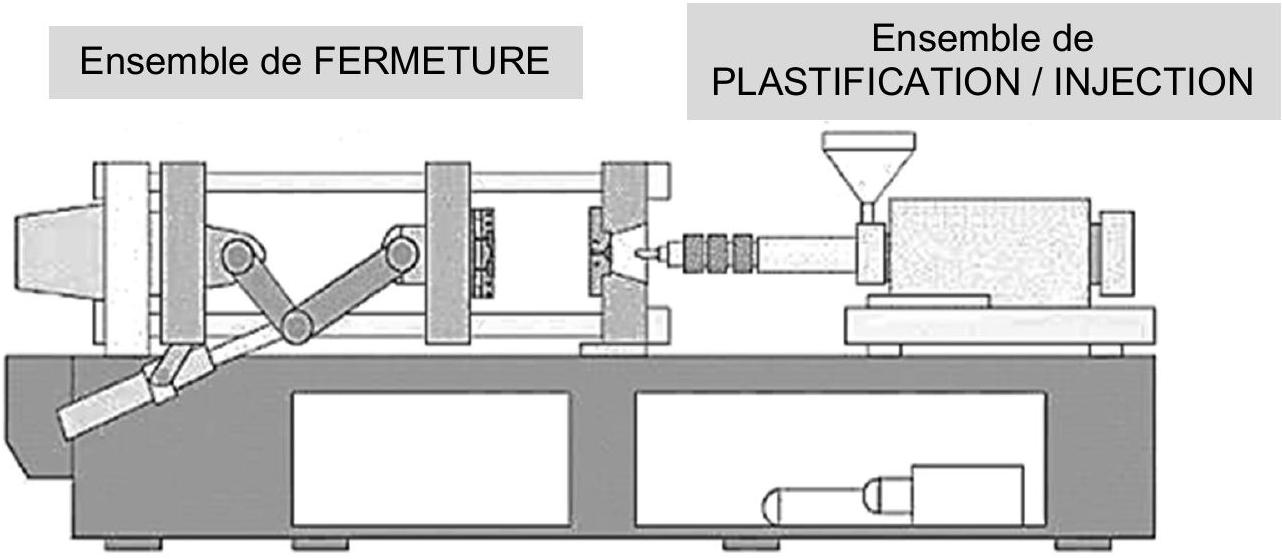
\includegraphics[alt={},max width=\textwidth]{076c1ba0-5a37-41d5-876a-83fc91dd5c32-04_559_1282_1315_454}
\captionsetup{labelformat=empty}
\caption{Figure 2 : Ensemble de fermeture et de plastification/injection}
\end{center}
\end{figure}

Une fois que la pièce est formée dans le moule, un système d'éjection pneumatique ou mécanique va faire tomber la pièce dans un bac ou sur un convoyeur sous l'ensemble de fermeture. Autre solution, un robot de déchargement, visible en figure 1, peut venir saisir les pièces dans le moule pour automatiser le conditionnement.

\subsection*{1.4. Processus de fabrication}
La fabrication d'une pièce en plastique par injection se déroule en différentes phases illustrées en figure 3. Durant ces phases, le fourreau est chauffé en permanence pour maintenir la matière sous forme liquide à la bonne température :

\begin{itemize}
  \item[-] Phase 1 : le moule est fermé, la vis tourne ce qui permet à la matière première d'entrer dans le fourreau et de chauffer. La rotation de la vis permet aussi d'homogénéiser la matière qui va s'accumuler à l'extrémité de la vis. Ainsi la vis recule au fur et à mesure. C'est la phase de plastification et dosage.
\end{itemize}

\begin{itemize}
  \item[-] Phase 2 : une fois qu'il y a suffisamment de matière en bout de vis, un vérin pousse sur la vis et la matière est alors injectée dans le moule. Un clapet anti-retour en bout de vis empêche la matière de remonter dans celle-ci. C'est la phase d'injection.
  \item[-] Phase 3 : la matière est maintenue sous pression dans le moule pendant que celui-ci refroidit, et elle va alors durcir. C'est la phase de refroidissement.
  \item[-] Phase 4 : la vis effectue un léger retrait pour libérer la pression sur la matière et ne plus en injecter. Le moule s'ouvre pour libérer la pièce. C'est la phase de démoulage et éjection.
\end{itemize}

Un nouveau cycle peut alors commencer pour fabriquer une nouvelle pièce.

\begin{figure}[h]
\begin{center}
  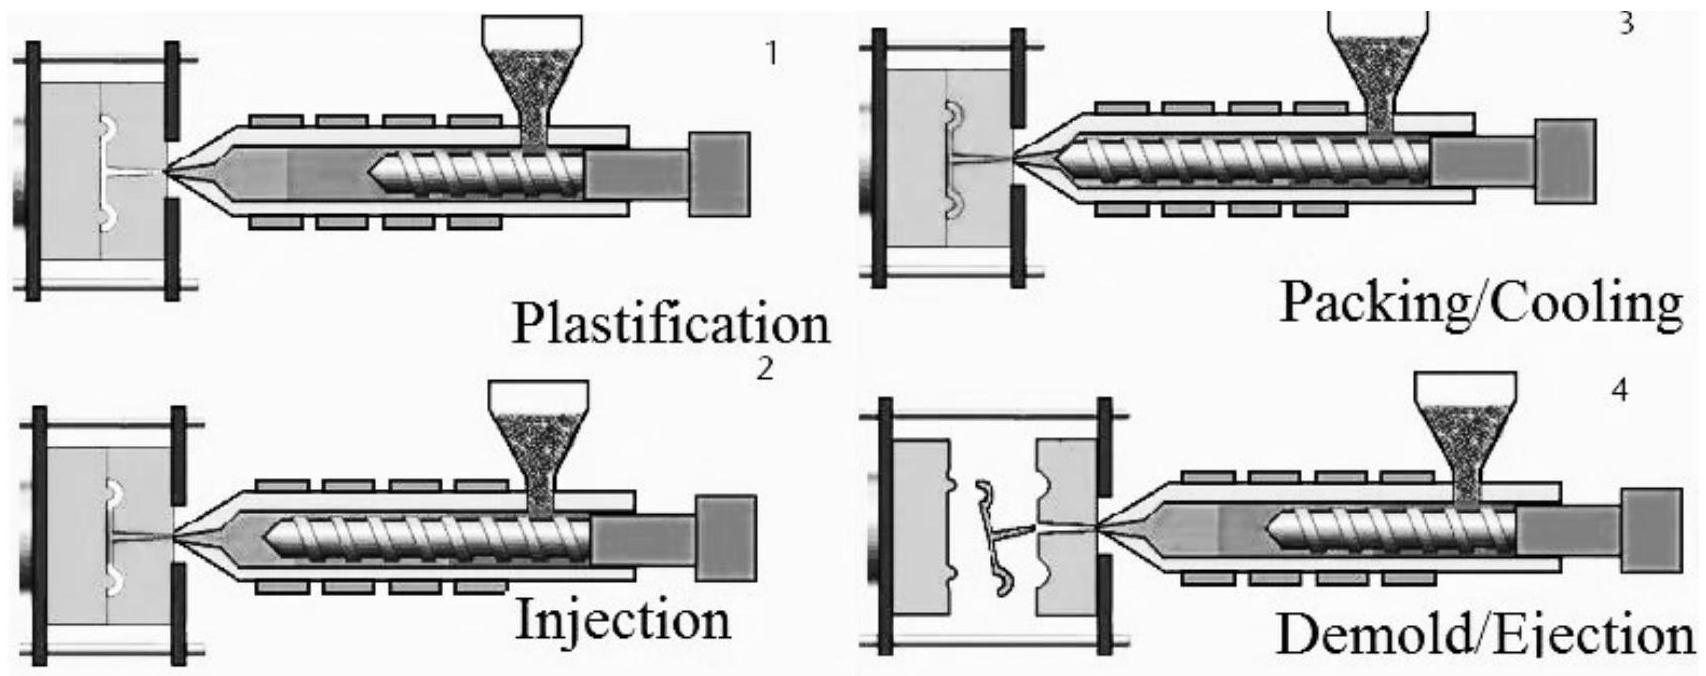
\includegraphics[alt={},max width=\textwidth]{076c1ba0-5a37-41d5-876a-83fc91dd5c32-05_676_1706_734_180}
\captionsetup{labelformat=empty}
\caption{Figure 3 : Phases de fabrication par injection plastique}
\end{center}
\end{figure}

\section*{1.5. Étude proposée}
L'étude proposée dans ce sujet est séparée en 8 parties indépendantes, pouvant également être séparées en sous-parties indépendantes. Enfin, certaines questions sont aussi indépendantes.

\begin{itemize}
  \item[-] Etude de la cadence de fabrication
  \item[-] Etude géométrique et cinématique
  \item[-] Etude des liaisons
  \item[-] Dimensionnement du moteur
  \item[-] Vérification des coussinets
  \item[-] Asservissement en température du fourreau
  \item[-] Alimentation de la machine d'entraînement de la vis du fourreau
  \item[-] Protocole de communication module moteur capteur du robot de déchargement
\end{itemize}

Un diagramme des exigences partiel est proposé en annexe 1.

\section*{PARTIE 2. ETUDE DE LA CADENCE DE FABRICATION}
Objectif : vérifier la capacité du système à respecter la cadence maximale souhaitée.\\
Pour évaluer la durée d'un cycle de fabrication, on décompose ce dernier en 4 étapes distinctes qui ont lieu les unes après les autres (pas de chevauchement) :

\begin{itemize}
  \item[1)] Fermeture du moule
  \item[2)] Injection plastique (la phase préalable de plastification/dosage est réalisée en temps masqué, donc non prise en compte dans le calcul du temps total)
  \item[3)] Ouverture du moule
  \item[4)] Ejection des pièces moulées
\end{itemize}

Le moule utilisé permet la fabrication simultanée de 10 pièces (donc en un seul cycle).\\
Question 1. Déterminer le temps moyen $t_{\text {moy }}$ (en secondes) d'un cycle de fabrication que doit réaliser la presse à injection pour respecter la cadence maximale précisée dans l'exigence "112 ".

\subsection*{2.1. Etude de l'étape d'injection}
Le temps d'injection des 10 pièces est noté $t_{i}$. Pour simplifier, les temps de maintien de la pression, de refroidissement et de solidification sont inclus dans le temps d'injection.\\
La vis a tourné, ce qui a permis à la matière première d'entrer dans le fourreau et de chauffer. La matière s'est accumulée à l'extrémité de la vis (figure 4), cette dernière ayant reculé au fur et à mesure.

\begin{figure}[h]
\begin{center}
  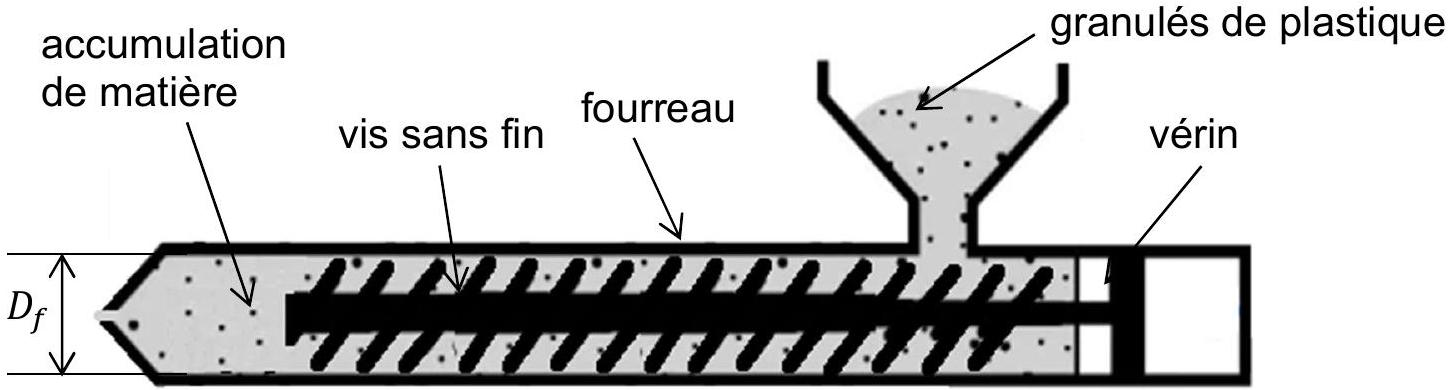
\includegraphics[alt={},max width=\textwidth]{076c1ba0-5a37-41d5-876a-83fc91dd5c32-06_390_1451_1463_370}
\captionsetup{labelformat=empty}
\caption{Figure 4 : Vue d'ensemble du système d'injection}
\end{center}
\end{figure}

Une fois qu'il y a suffisamment de matière en bout de vis, un vérin pousse sur la vis qui agit ainsi comme un piston : c'est la phase d'injection. Le diamètre intérieur du fourreau est noté $D_{f}=0,04 m$, la vitesse d'injection (vitesse de translation de la vis) vaut $v_{i}=0,12 m / s$.

Question 2. Déterminer l'expression littérale du débit d'injection $Q_{i}$ puis calculer sa valeur numérique en $c m^{3} / s$.

Le volume de matière nécessaire pour la fabrication simultanée des 10 pièces est évalué à $V_{p}=210 c m^{3}$.

Question 3. Déterminer la formule littérale du temps d'injection $t_{i}$ et faire l'application numérique.\\
2.2. Etude de l'étape d'éjection\\
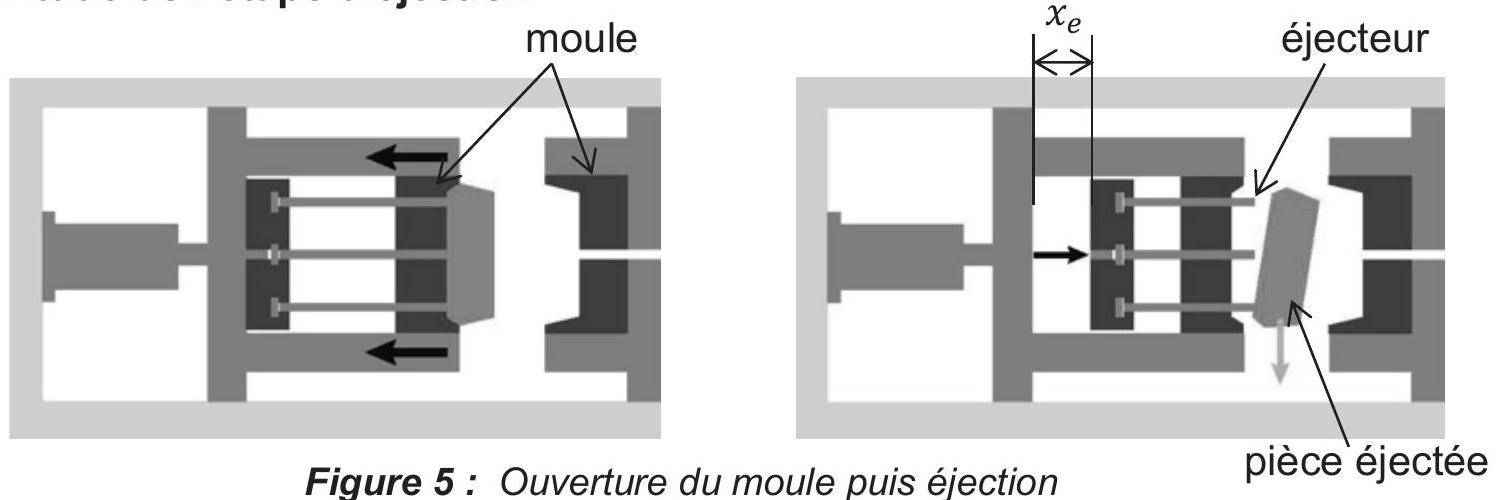
\includegraphics[max width=\textwidth, alt={}, center]{076c1ba0-5a37-41d5-876a-83fc91dd5c32-07_500_1496_289_306}\\
Une fois l'ouverture du moule effectuée, les 10 composants sont éjectés simultanément en un temps d'éjection noté $t_{e}$. Les éjecteurs ont une course $x_{e}=0,15 m$ (figure 5) et une vitesse de déplacement $v_{e}=0,3 \mathrm{~m} / \mathrm{s}$ supposée constante durant toute la course. Ils décrivent un aller-retour avant la fermeture du moule.

Question 4. Déterminer la formule littérale du temps d'éjection $t_{e}$ et faire l'application numérique.\\
2.3. Etude des étapes d'ouverture et de fermeture du moule\\
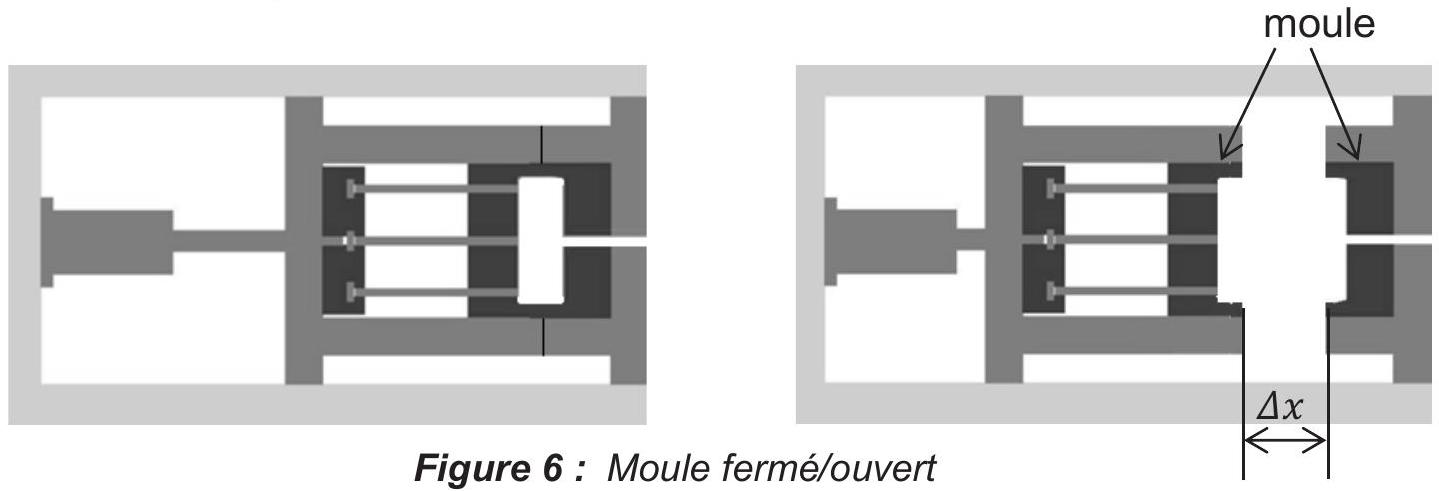
\includegraphics[max width=\textwidth, alt={}, center]{076c1ba0-5a37-41d5-876a-83fc91dd5c32-07_491_1439_1294_313}\\
Pour l'application étudiée, on suppose que le moule doit être déplacé sur une distance $\Delta x=0,432 m$. Pour l'ouverture, comme pour la fermeture, on impose des lois de mouvement en trapèze (3 phases) pour le paramètre de vitesse $\dot{x}$, avec égalité des temps d'accélération et de décélération. On se place dans la situation où les accélérations et les décélérations sont constantes et maximales :

$$
\left.\begin{array}{l}
\ddot{x}_{\max }=a_{\max }=1 \mathrm{~m} / \mathrm{s}^{2} \\
\dot{x}_{\max }=v_{\max }=0,6 \mathrm{~m} / \mathrm{s}
\end{array} \quad \text { (vitesse atteinte en fin de phase } 1\right)
$$

Question 5. Proposer un tracé représentant l'allure de l'évolution de la vitesse de déplacement du moule en phase de fermeture (ou d'ouverture) en fonction du temps $\dot{x}=f(t)$.\\
Question 6. Calculer la durée minimale $\mathrm{t}_{\text {o/f }}$ de la phase de fermeture (ou d'ouverture) du moule.\\
2.4. Etude d'un cycle complet

Question 7. Déterminer la formule littérale de la durée $\mathrm{t}_{\text {cycl }}$ d'un cycle de fabrication d'un lot de 10 pièces et faire l'application numérique.

Question 8. Conclure sur la capacité du système à respecter la cadence maximale.

\section*{PARTIE 3. ETUDE GEOMETRIQUE ET CINEMATIQUE}
Objectifs : pré-dimensionner en vitesse le moteur de l'unité de fermeture du moule et vérifier une donnée constructeur.

L'unité de fermeture du moule est constituée d'un mécanisme à genouillère dont le schéma cinématique complet ainsi que le fonctionnement sont décrits dans les annexes 2 et 3. Le schéma cinématique plan retenu pour l'étude géométrique est le suivant (figure 7) :

\begin{figure}[h]
\begin{center}
  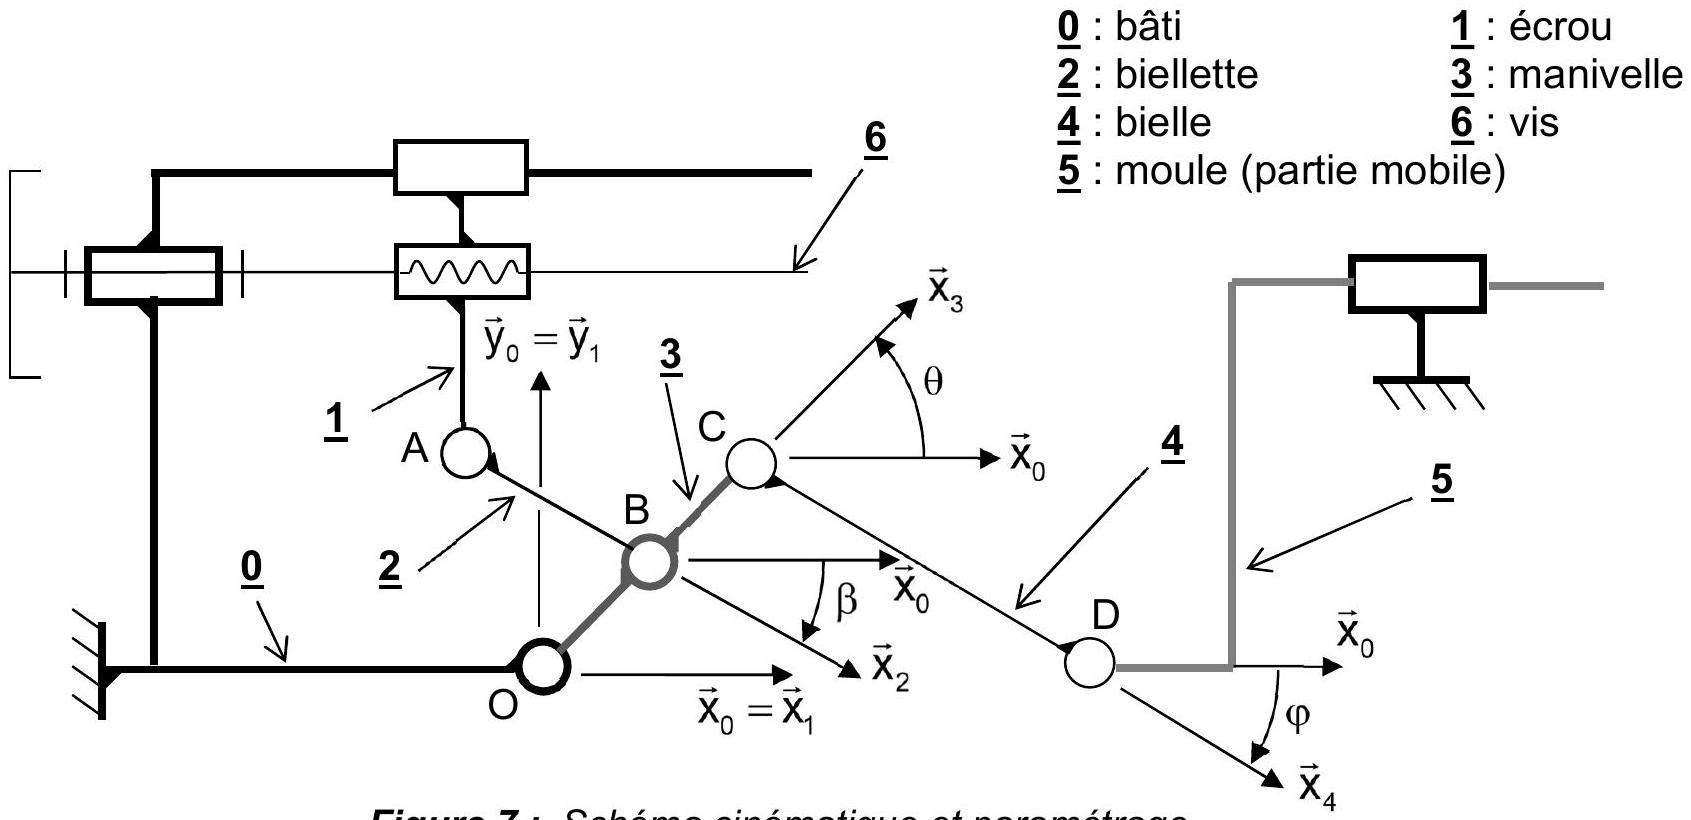
\includegraphics[alt={},max width=\textwidth]{076c1ba0-5a37-41d5-876a-83fc91dd5c32-08_820_1691_693_209}
\captionsetup{labelformat=empty}
\caption{Figure 7 : Schéma cinématique et paramétrage}
\end{center}
\end{figure}

On donne :

\begin{itemize}
  \item[-] $\overrightarrow{O A}=\lambda \cdot \vec{x}_{0}+h \cdot \vec{y}_{0} \quad$ avec $\lambda$ un paramètre algébrique (peut être $\geq 0$ ou $\leq 0$ )
  \item[-] $\overrightarrow{O B}=e . \vec{x}_{3}$
  \item[-] $\overrightarrow{A B}=d . \vec{x}_{2}$
  \item[-] $\overrightarrow{O C}=2 e . \vec{x}_{3}$
  \item[-] $\overrightarrow{C D}=L . \vec{x}_{4}$
  \item[-] $\beta=\left(\vec{x}_{0}, \vec{x}_{2}\right)=\left(\vec{y}_{0}, \vec{y}_{2}\right)$
  \item[-] $\theta=\left(\vec{x}_{0}, \vec{x}_{3}\right)=\left(\vec{y}_{0}, \vec{y}_{3}\right)$
  \item[-] $\varphi=\left(\vec{x}_{0}, \vec{x}_{4}\right)=\left(\vec{y}_{0}, \vec{y}_{4}\right)$
\end{itemize}

\subsection*{3.1. Etude géométrique générale}
Question 9. Réaliser les figures de changements de bases mettant en évidence les paramètres angulaires.

Question 10. Ecrire une équation vectorielle de fermeture géométrique sur le cycle OABO. En projetant sur $\vec{x}_{0}$ et $\vec{y}_{0}$, en déduire les deux équations scalaires liant les paramètres $\lambda$, $\theta$ et $\beta$.

Question 11. A partir des deux équations précédemment obtenues, établir une relation scalaire ne contenant plus l'angle $\beta$ et montrer qu'elle peut se mettre sous la forme suivante :

$$
P \cdot \cos \theta+Q \cdot \sin \theta=R
$$

en précisant les expressions de P, Q et R.

Le terme $P^{2}+Q^{2}$ ne s'annulant jamais, la relation précédente peut aussi s'écrire :

$$
\frac{P}{\sqrt{P^{2}+Q^{2}}} \cdot \cos \theta+\frac{Q}{\sqrt{P^{2}+Q^{2}}} \cdot \sin \theta=\frac{R}{\sqrt{P^{2}+Q^{2}}}
$$

On pose : $\cos \psi=\frac{P}{\sqrt{P^{2}+Q^{2}}}$ et $\sin \psi=\frac{Q}{\sqrt{P^{2}+Q^{2}}}$\\
On rappelle que, pour x et y réels : $\cos (x-y)=\cos x . \cos y+\sin x . \sin y$\\
Question 12. Exprimer $\theta$ en fonction $\mathrm{de} \mathrm{P}, \mathrm{Q}$ et R .

\subsection*{3.2. Prédimensionnement en vitesse du moteur}
L'expression trouvée précédemment étant trop complexe à exploiter, on fournit un tracé de la fonction $\theta=\mathrm{f}(\lambda)$ sur la figure 8.

\begin{figure}[h]
\begin{center}
  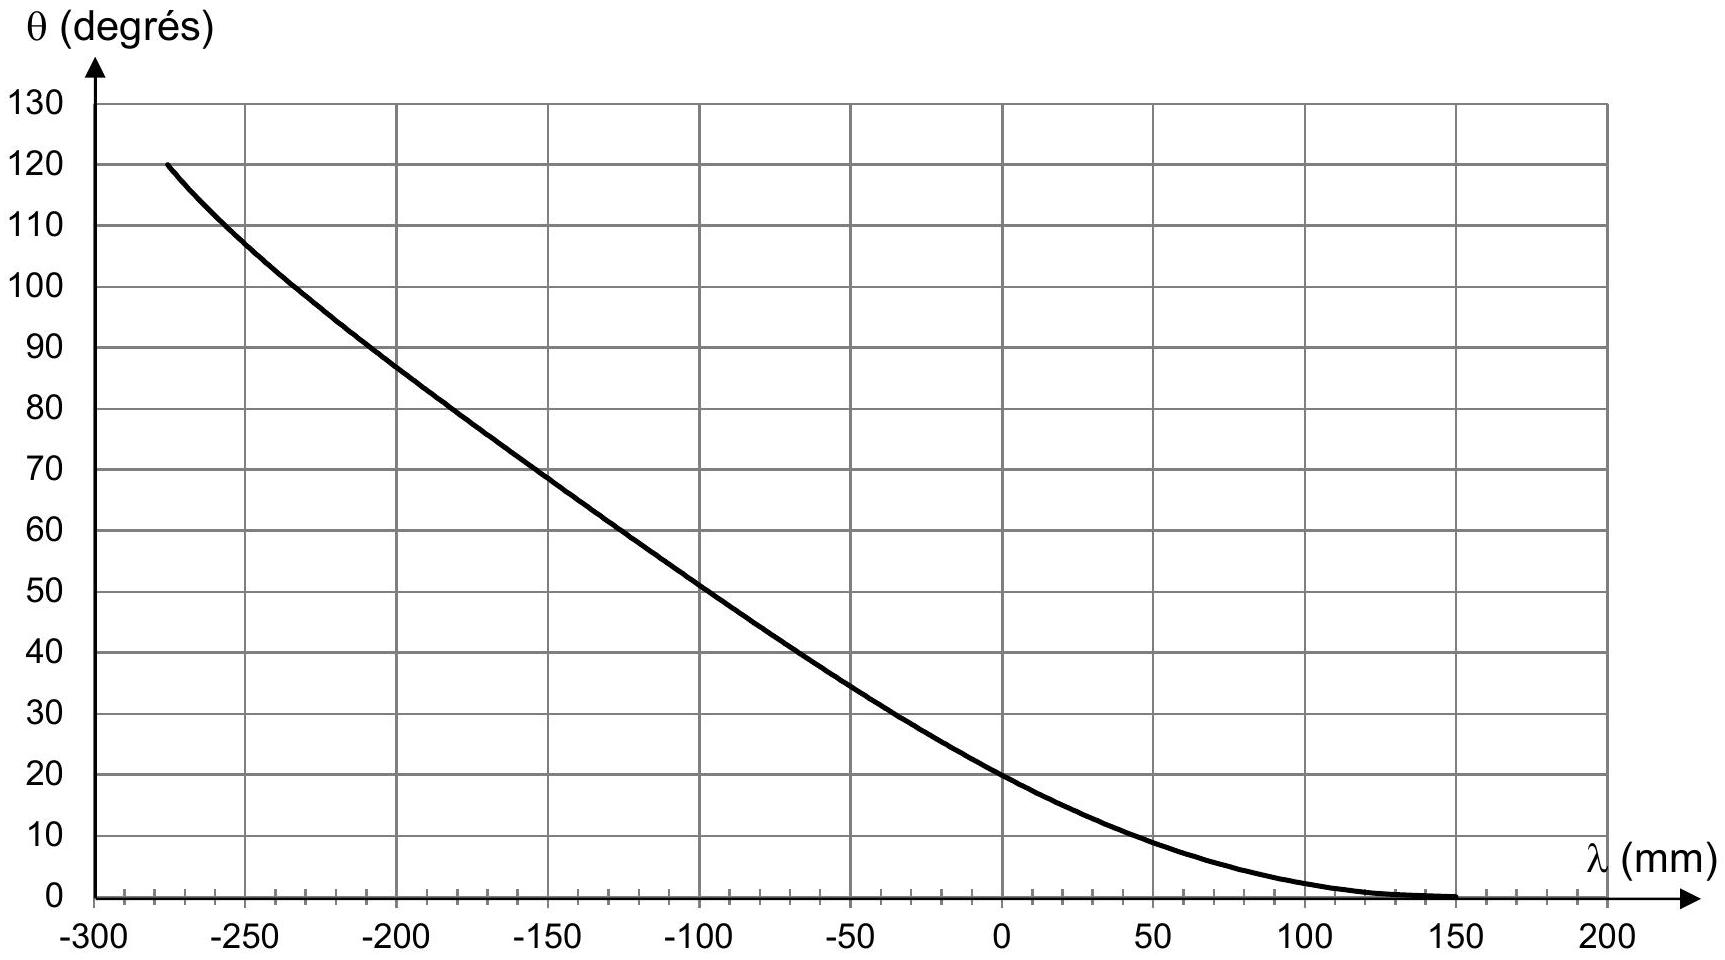
\includegraphics[alt={},max width=\textwidth]{076c1ba0-5a37-41d5-876a-83fc91dd5c32-09_960_1725_1287_204}
\captionsetup{labelformat=empty}
\caption{Figure 8 : Tracé de la fonction $\theta=\mathrm{f}(\lambda)$}
\end{center}
\end{figure}

Lorsque le moule est en position fermée, l'angle $\theta$ vaut $\theta=0^{\circ}$.\\
Lorsque le moule est en position ouverte, l'angle $\theta$ vaut $\theta=90^{\circ}$.

Question 13. Déterminer $\Delta \lambda$, l'amplitude du déplacement horizontal de la pièce 1 lors d'une ouverture (ou fermeture) de moule.

Question 14. Exprimer puis calculer en $m / s$ la vitesse moyenne $\dot{\lambda}_{\text {moy }}$ de déplacement de la pièce 1 si on souhaite que ce déplacement soit effectué en un temps $\Delta t=1,2 s$ (on néglige ici les phases d'accélération et de décélération).

Le dispositif d'entraînement en translation de l'écrou 1 est constitué d'un moteur électrique, d'une transmission poulies/courroie crantées et d'un système vis/écrou $\underline{\mathbf{6}} / \mathbf{1}$ dont le pas vaut $p_{v}=0,03 m / t r$ (voir figure 9).

On note $\mathrm{N}_{\mathrm{m}}$ la vitesse de rotation du moteur et $\mathrm{N}_{6 / 0}$ la vitesse de rotation de la vis $\underline{6}$ par rapport au bâti 0. Ces vitesses sont exprimées en $\mathrm{tr} / \mathrm{min}$.

\begin{figure}[h]
\begin{center}
  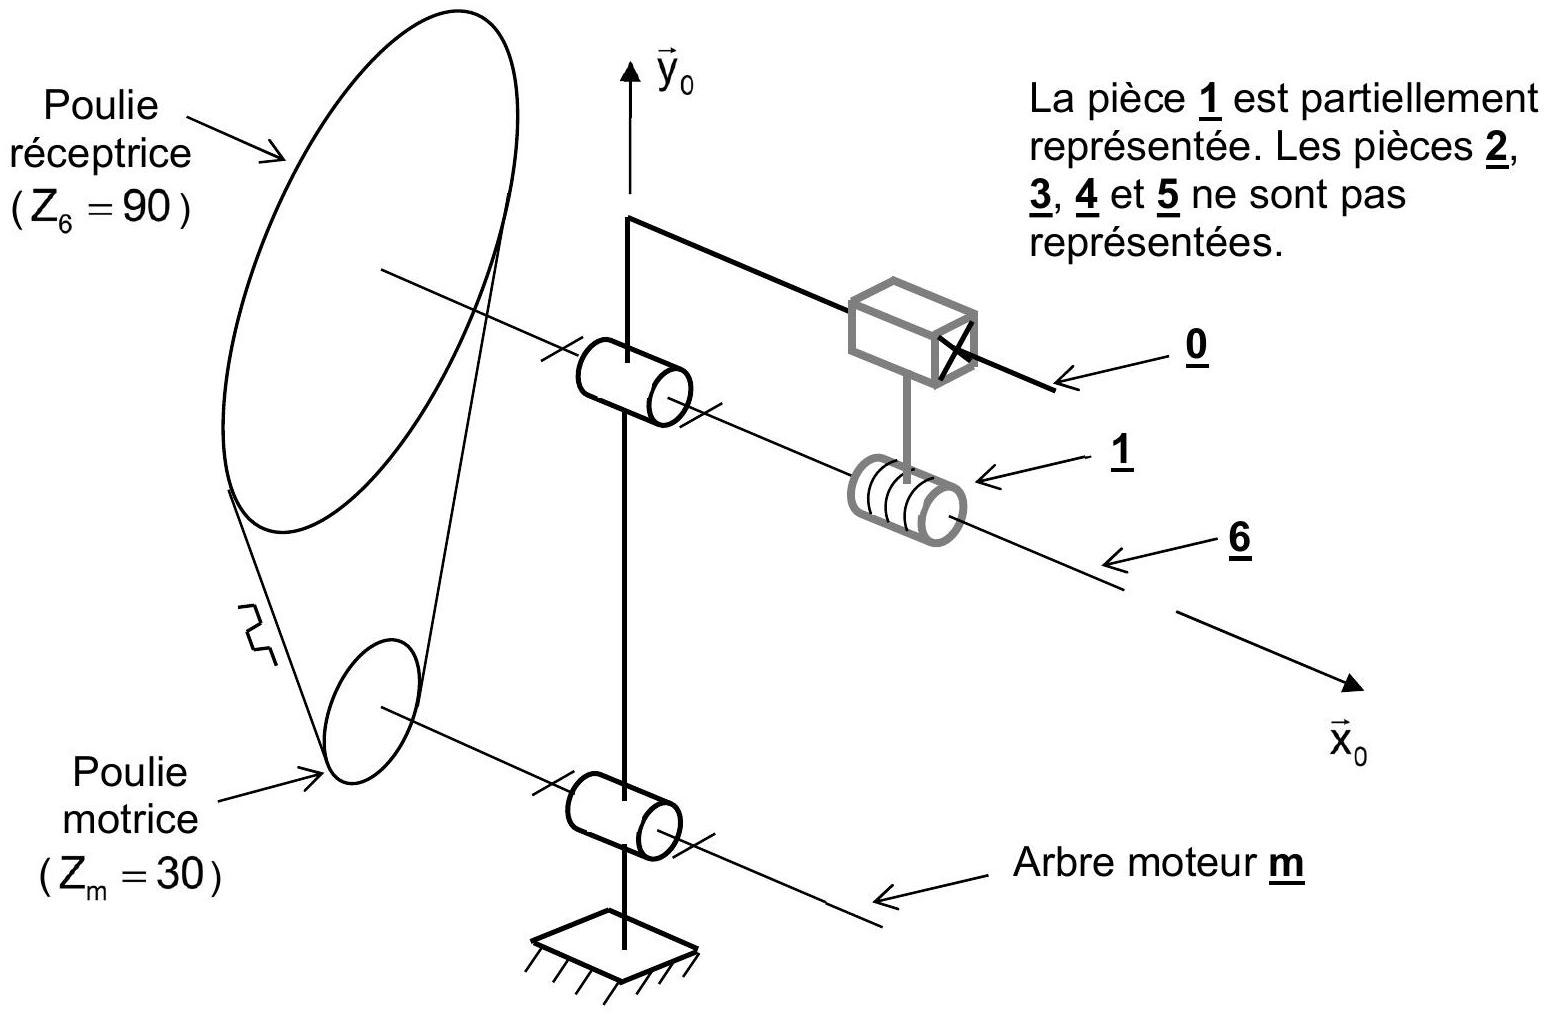
\includegraphics[alt={},max width=\textwidth]{076c1ba0-5a37-41d5-876a-83fc91dd5c32-10_1015_1549_1131_284}
\captionsetup{labelformat=empty}
\caption{Figure 9 : Schéma de la transmission de puissance}
\end{center}
\end{figure}

Question 15. Etablir la relation entre la vitesse moyenne $\dot{\lambda}_{\text {moy }}$ de déplacement de la pièce 1 et la vitesse de rotation $\mathrm{N}_{6 / 0}$ de la vis $\underline{6}$ en faisant intervenir le pas $\mathrm{p}_{\mathrm{v}}$ du système vis/écrou 6/1.

Question 16. Exprimer la vitesse de rotation $N_{m}$ du moteur en fonction de $N_{6 / 0}, Z_{6}$ et $Z_{m}$. En déduire $\mathrm{N}_{\mathrm{m}}$ en fonction de $\dot{\lambda}_{\text {moy }}, \mathrm{p}_{\mathrm{v}}, \mathrm{Z}_{6}$ et $\mathrm{Z}_{\mathrm{m}}$. Calculer la valeur numérique de $\mathrm{N}_{\mathrm{m}}$ (en $\mathrm{tr} / \mathrm{min}$ ) permettant d'obtenir l'ouverture du moule dans le temps souhaité.

\subsection*{3.3. Détermination de l'amplitude d'ouverture du moule}
Une grande ouverture du moule est intéressante pour la fabrication car cela libère de l'espace pour l'éjection de pièces ayant une profondeur élevée.

L'angle $\theta$ précédemment exprimé intervient dans le système de transformation de mouvement de type bielle-manivelle constitué des pièces $\underline{\mathbf{3}}$, $\underline{\mathbf{4}}$ et $\underline{\mathbf{5}}$. Les positions extrêmes du moule $\mathbf{5}$ sont obtenues pour $\theta=0^{\circ}$ et $\theta=90^{\circ}$.

On donne les valeurs numériques suivantes :

$$
e=150 \mathrm{~mm} \quad L=400 \mathrm{~mm}
$$

Question 17. A partir de l'étude du triangle OCD (figure 7) pour $\theta=90^{\circ}$, déterminer l'expression puis la valeur numérique de $\|\overrightarrow{O D}\|$.

Question 18. En menant une étude similaire, déterminer l'expression puis la valeur numérique de $\|\overrightarrow{O D}\|$ pour $\theta=0^{\circ}$. En déduire l'amplitude $\Delta x$ d'ouverture du moule $\underline{\mathbf{5}}$. Conclure quant au respect de l'exigence '1211'.

\section*{PARTIE 4. ETUDE DES LIAISONS}
Objectif : analyser la solution de guidage de l'écrou 1.\\
Lorsqu'on regarde en détail la solution constructive, l'écrou 1 est en fait guidé par rapport au bâti 0 à l'aide de 2 liaisons cinématiques en J et K. Le schéma d'architecture de la figure 10 montre la disposition de ces liaisons.

\begin{figure}[h]
\begin{center}
  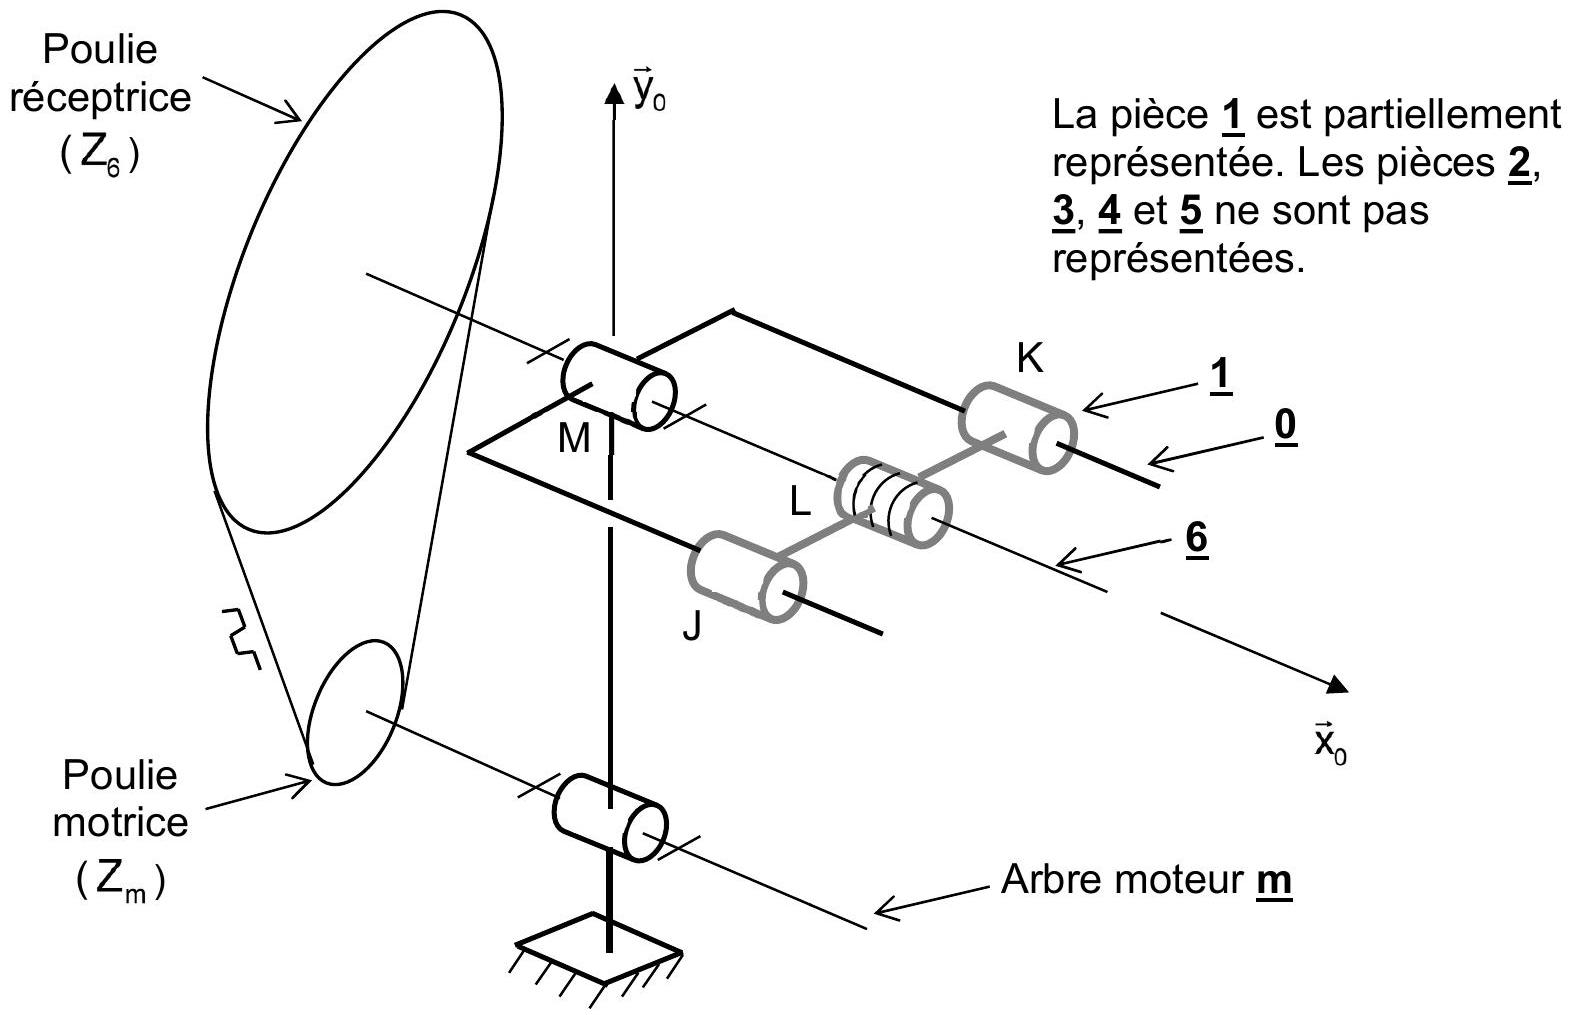
\includegraphics[alt={},max width=\textwidth]{076c1ba0-5a37-41d5-876a-83fc91dd5c32-12_1015_1573_678_248}
\captionsetup{labelformat=empty}
\caption{Figure 10 : Schéma d'architecture du guidage de l'écrou}
\end{center}
\end{figure}

Question 19. Proposer un graphe de structure faisant intervenir les pièces Q, 1 et 6. Les liaisons identifiées entre les solides 0 et 1 sont-elles en série ou en parallèle ?

On se propose de vérifier la nature de la liaison équivalente entre les solides 0 et 1 à partir de l'écriture des torseurs statiques ou cinématiques associés aux liaisons identifiées à la question précédente.

Donnée : $\overrightarrow{K L}=\overrightarrow{L J}=a \cdot \vec{z}_{0}$

Pour l'écriture des torseurs, on pourra utiliser les notations suivantes, en les adaptant à l'exercice :

\begin{itemize}
  \item[-] pour un torseur statique :
$$
\left\{T_{1 \rightarrow 2}\right\}=\left\{\begin{array}{ll}
X_{E} & L_{E} \\
Y_{E} & M_{E} \\
Z_{E} & N_{E}
\end{array}\right\}_{\left(\vec{x}_{0}, \vec{y}_{0}, \vec{z}_{0}\right)}=\left\{\begin{array}{l}
\vec{R}_{1 \rightarrow 2}=X_{E} \cdot \vec{x}_{0}+Y_{E} \cdot \vec{y}_{0}+Z_{E} \cdot \vec{z}_{0} \\
\vec{M}_{E, 1 \rightarrow 2}=L_{E} \cdot \vec{x}_{0}+M_{E} \cdot \vec{y}_{0}+N_{E} \cdot \vec{z}_{0}
\end{array}\right\}
$$
  \item[-] pour un torseur cinématique :
$$
\left\{V_{2 / 1}\right\}=\left\{\begin{array}{ll}
\omega_{1} & V_{1} \\
\omega_{2} & V_{2} \\
\omega_{3} & V_{3}
\end{array}\right\}_{\left(\vec{x}_{0}, \vec{y}_{0}, \vec{z}_{0}\right)}=\left\{\begin{array}{l}
\vec{\Omega}_{2 / 1}=\omega_{1} \cdot \vec{x}_{0}+\omega_{2} \cdot \vec{y}_{0}+\omega_{3} \cdot \vec{z}_{0} \\
\vec{v}_{E \in 2 / 1}=v_{1} \cdot \vec{x}_{0}+v_{2} \cdot \vec{y}_{0}+v_{3} \cdot \vec{z}_{0}
\end{array}\right\}
$$
\end{itemize}

Question 20. Ecrire le torseur statique ${ }_{\mathrm{K}}\left\{\mathrm{T}_{0 \rightarrow 1}\right\}$ et le torseur cinématique ${ }_{\mathrm{K}}\left\{\mathrm{V}_{1 / 0}\right\}$ de la liaison au point K entre les solides 0 et 1.

Question 21. Par une méthode au choix, déterminer soit le torseur statique, soit le torseur cinématique de la liaison équivalente aux 2 liaisons en J et K. En déduire le nom et les caractéristiques de la liaison équivalente entre les solides 0 et 1.

\section*{PARTIE 5. DIMENSIONNEMENT DU MOTEUR}
Objectif : pré-dimensionner en couple le moteur de l'unité de fermeture du moule.\\
L'unité de fermeture du moule 5 est motorisée par une machine synchrone.\\
Quand on parle du moule $\underline{\mathbf{5}}$, il s'agit de la partie mobile du moule puisque l'autre partie est fixée au bâti et ne bouge donc pas. La figure 11 rappelle la modélisation du système et les mouvements des pièces.

\begin{figure}[h]
\begin{center}
  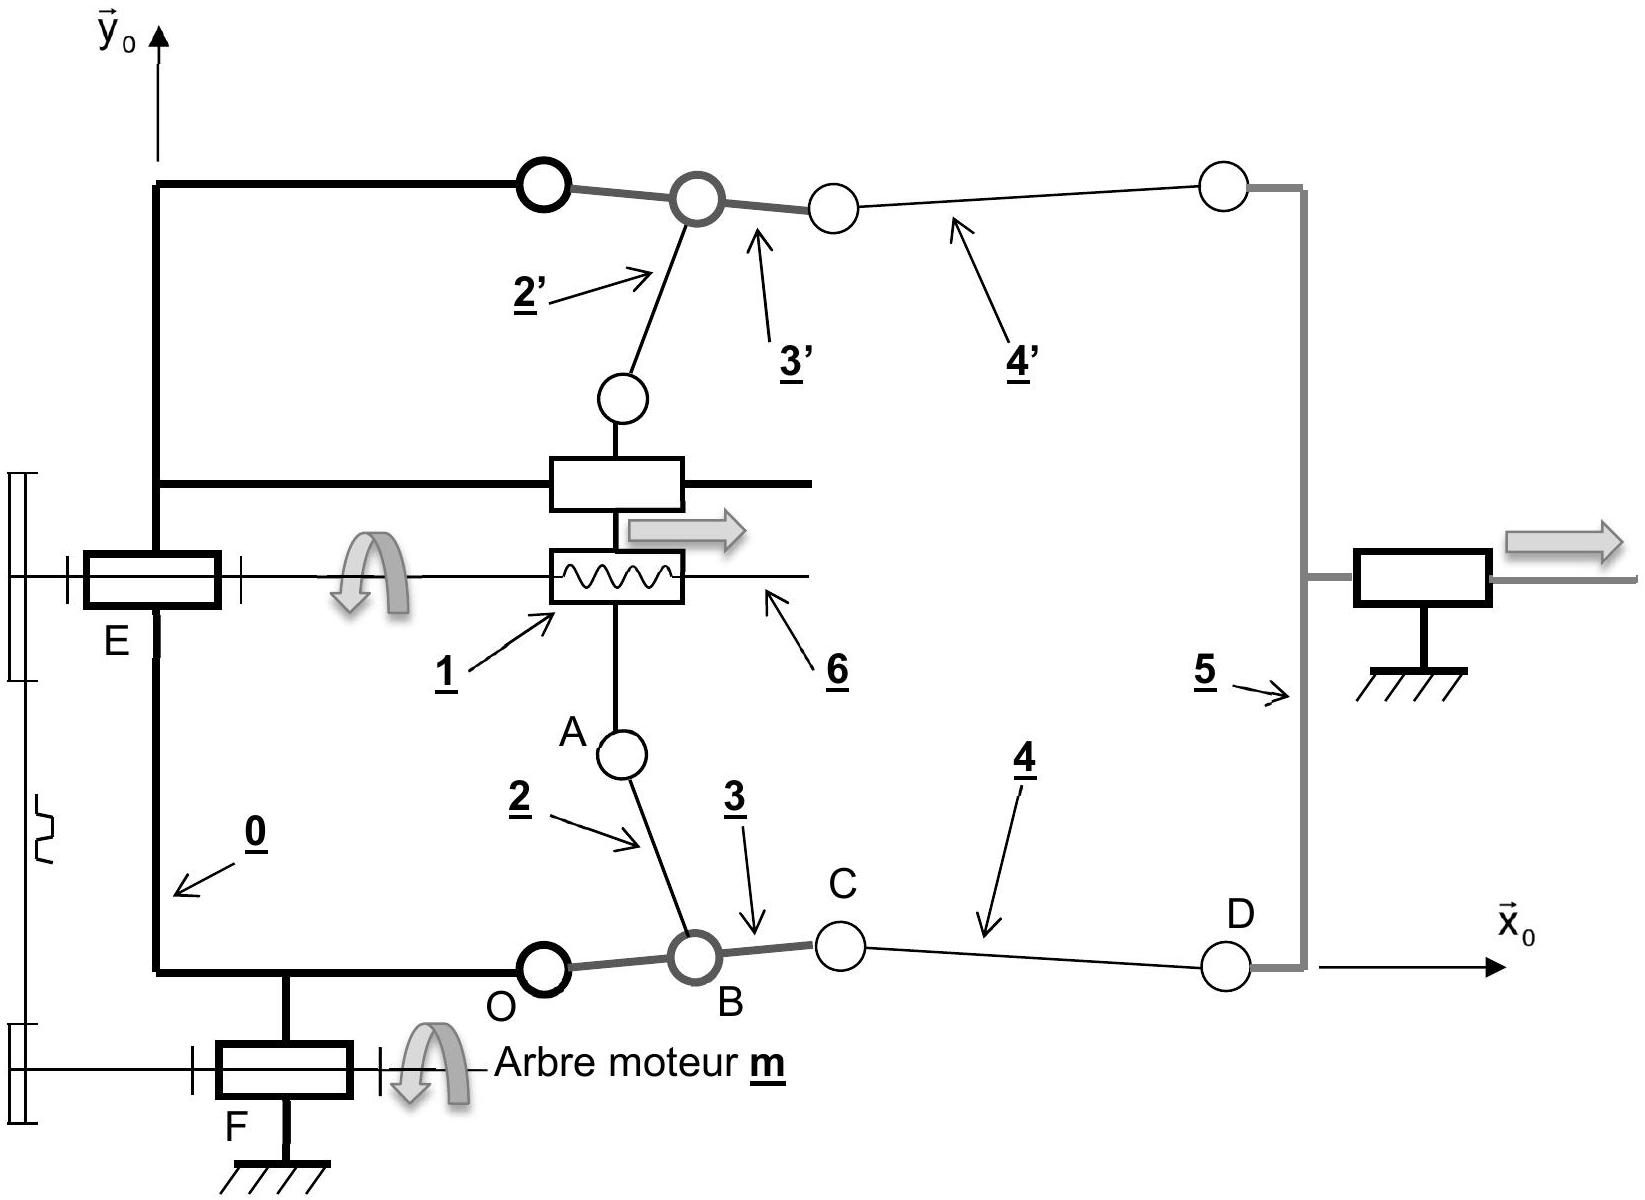
\includegraphics[alt={},max width=\textwidth]{076c1ba0-5a37-41d5-876a-83fc91dd5c32-14_1200_1645_666_236}
\captionsetup{labelformat=empty}
\caption{Figure 11 : Vue d'ensemble des différentes pièces}
\end{center}
\end{figure}

Pour effectuer un prédimensionnement du moteur, on fournit les données simplifiées suivantes :

\begin{itemize}
  \item[-] $J_{m}=15.10^{-3} \mathrm{~kg} . \mathrm{m}^{2}$ : moment d'inertie de l'arbre moteur $\underline{\mathbf{m}}$ autour de son axe de rotation
  \item[-] $\omega_{\mathrm{m}}$ : vitesse de rotation du moteur (en $\mathrm{rad} / \mathrm{s}$ )
  \item[-] $\mathrm{C}_{\mathrm{m}}$ : couple développé par le moteur
  \item[-] $\mathrm{J}_{\mathrm{v}}$ : moment d'inertie de la vis $\underline{6}$ autour de son axe de rotation
  \item[-] $\omega_{\mathrm{v}}$ : vitesse de rotation de la vis $\underline{6}$ (en $\mathrm{rad} / \mathrm{s}$ )
  \item[-] $\quad \mathrm{p}_{\mathrm{v}}$ : pas de la vis $\underline{6}$ (en $m / t r$ )
  \item[-] $\quad \dot{\lambda}$ : vitesse de translation selon $\vec{x}_{0}$ de la pièce 1 (en $m / s$ )
  \item[-] $\quad \dot{x}$ : vitesse de translation selon $\vec{x}_{0}$ du moule $\underline{\mathbf{5}}$ (en $m / s$ )
\end{itemize}

\begin{itemize}
  \item[-] $\mathrm{r}=\frac{\omega_{\mathrm{v}}}{\omega_{\mathrm{m}}}$ : rapport des vitesses de rotation de la transmission poulies/courroie
  \item[-] $\quad i=\frac{\dot{x}}{\dot{\lambda}}$ : rapport (supposé constant) des vitesses linéaires des pièces $\underline{1}$ et $\underline{5}$
  \item[-] Masses et inerties des pièces 1, 2, 2', 3, 3', 4 et 4' négligées
  \item[-] M : masse de la partie mobile du moule 5
  \item[-] Les liaisons sont parfaites, les rendements sont supposés égaux à 1.
  \item[-] Les autres pièces non citées sont négligées pour ce calcul.
  \item[-] Le repère associé au bâti $\underline{0}$ de la presse à injecter est supposé galiléen.
  \item[-] L'axe $\vec{y}_{0}$ correspond à la verticale terrestre : $\vec{g}=-g . \vec{y}_{0}$ avec $g=9,81 \mathrm{~m} / \mathrm{s}^{2}$
\end{itemize}

Le moment d'inertie autour de son axe de révolution d'un cylindre de masse m et de rayon R vaut $\mathrm{J}=\frac{\mathrm{m} . \mathrm{R}^{2}}{2}$.\\
La vis 6 est en acier de masse volumique $\rho$. Sa longueur est notée $\mathrm{L}_{\mathrm{v}}$, son diamètre moyen est noté $\mathrm{d}_{\mathrm{v}}$.

Question 22. En assimilant la vis $\underline{6}$ à un cylindre, exprimer son moment d'inertie $J_{\mathrm{v}}$ en fonction de ses caractéristiques dimensionnelles et de masse.

Question 23. Exprimer $\dot{x}$ en fonction de $\mathrm{p}_{\mathrm{v}}, \mathrm{r}, \mathrm{i}$ et $\omega_{\mathrm{m}}$.\\
Pour la suite, on pose $\dot{x}=k . \omega_{m}$ avec $\mathrm{k}=2,4.10^{-3} \mathrm{~m}$.\\
On isole l'ensemble $\mathrm{S}=\{$ axe moteur, $\underline{\mathbf{1}}, \underline{\mathbf{2}}, \underline{\mathbf{3}}, \underline{\mathbf{4}}, \underline{\mathbf{5}}, \underline{\mathbf{6}}\}$\\
Question 24. Exprimer l'énergie cinétique $\mathrm{E}_{\mathrm{C}(\mathrm{S} / 0)}$ de l'ensemble S en fonction de $\omega_{\mathrm{m}}$. En déduire l'expression de l'inertie équivalente $\mathrm{J}_{\mathrm{eq}}$ ramenée à l'arbre moteur.

Question 25. Faire le bilan des puissances extérieures et intérieures à l'ensemble S .

Question 26. Appliquer le théorème de l'énergie cinétique au système isolé et en déduire l'équation faisant intervenir le couple moteur $\mathrm{C}_{\mathrm{m}}$, l'inertie équivalente $\mathrm{J}_{\mathrm{eq}}$ et l'accélération angulaire du moteur $\dot{\omega}_{\mathrm{m}}$.

On souhaite imposer une accélération $\ddot{x}=1 \mathrm{~m} / \mathrm{s}^{2}$ au moule $\underline{\mathbf{5}}$. On prendra $\mathrm{J}_{\text {eq }}=2.10^{-2} \mathrm{~kg} . \mathrm{m}^{2}$\\
Question 27. Déterminer la valeur du couple moteur $\mathrm{C}_{\mathrm{m}}$ permettant d'atteindre l'accélération $\ddot{x}$ souhaitée.

Pour la suite, on donne les caractéristiques nominales suivantes pour le moteur :

$$
\mathrm{N}_{\mathrm{m}}=1900 \mathrm{tr} / \mathrm{min} \quad \mathrm{C}_{\mathrm{m}}=9 \mathrm{~N} . \mathrm{m}
$$

Question 28. A partir de l'annexe 4, proposer une référence de moteur dont les caractéristiques nominales conviennent.

\section*{PARTIE 6. VERIFICATION DES COUSSINETS}
Objectif : vérifier le dimensionnement des éléments de guidage en rotation.\\
En phase de fermeture, les 4 bielles $\underline{\mathbf{4}}$ agissent sur la partie mobile du moule $\mathbf{5}$ pour réaliser la fermeture de ce dernier (figure 12). Les liaisons pivots en A, B, C, et D utilisent des bagues de frottement (ou coussinets). Ces dernières doivent être correctement dimensionnées pour éviter une dégradation rapide des articulations.

\begin{figure}[h]
\begin{center}
  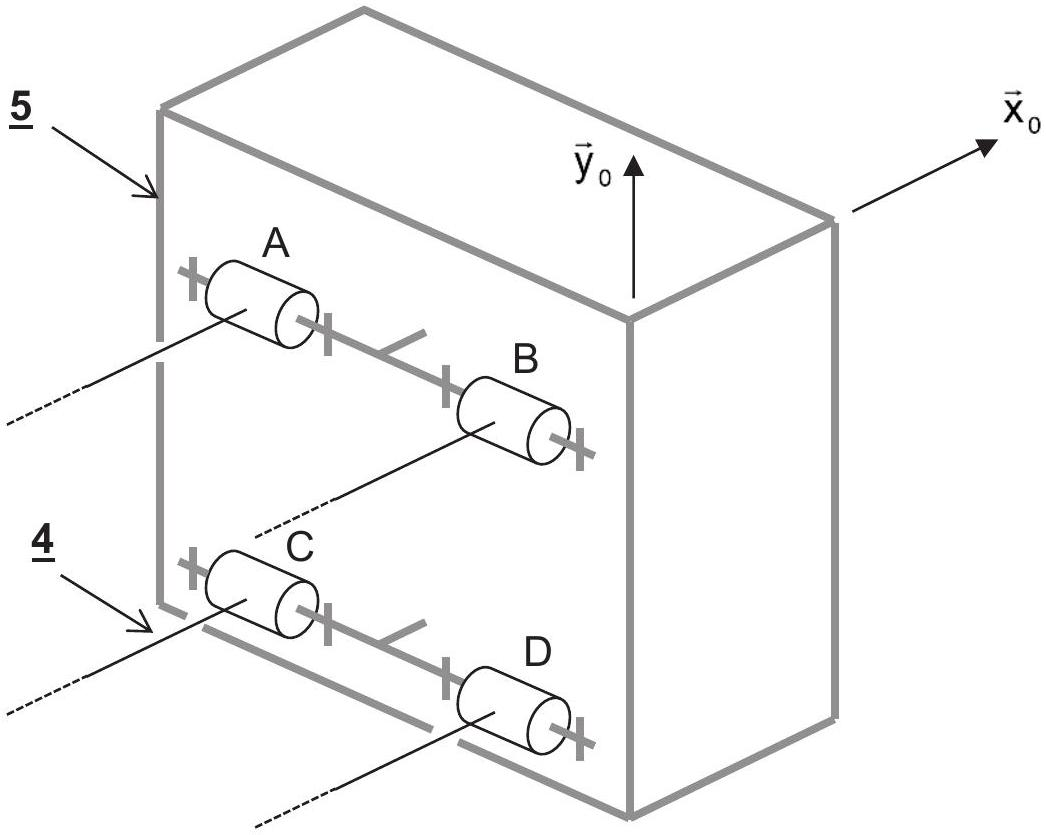
\includegraphics[alt={},max width=\textwidth]{076c1ba0-5a37-41d5-876a-83fc91dd5c32-16_835_1046_645_599}
\captionsetup{labelformat=empty}
\caption{Figure 12 : Schéma de principe}
\end{center}
\end{figure}

Chaque bielle 4 comporte un coussinet à son extrémité en contact avec le moule $\underline{\mathbf{5}}$, donc au niveau des liaisons en A, B, C et D.

On fournit les caractéristiques suivantes pour les coussinets utilisés :

\begin{itemize}
  \item[-] Diamètre intérieur : $d_{i n t}=75 \mathrm{~mm}$
  \item[-] Diamètre extérieur : $\mathrm{D}_{\text {ext }}=85 \mathrm{~mm}$
  \item[-] Longueur : $\mathrm{b}=80 \mathrm{~mm}$
\end{itemize}

\begin{center}
\begin{tabular}[t]{|l|l|l|l|}
\hline
\multirow{2}{*}{Pression admissible} & Charge : statique & \multirow{2}{*}{$\mathrm{p}_{\text {max }}$} & $200 \mathrm{~N} / \mathrm{mm}^{2}$ \\
\hline
 & Charge : rotation, oscillation &  & $140 \mathrm{~N} / \mathrm{mm}^{2}$ \\
\hline
\multicolumn{2}{|l|}{Vitesse de glissement admissible} & $\mathrm{v}_{\text {max }}$ & $200 \mathrm{~mm} / \mathrm{s}$ \\
\hline
\end{tabular}
\end{center}

\subsection*{6.1. Vérification de la pression admissible}
\begin{figure}[h]
\begin{center}
  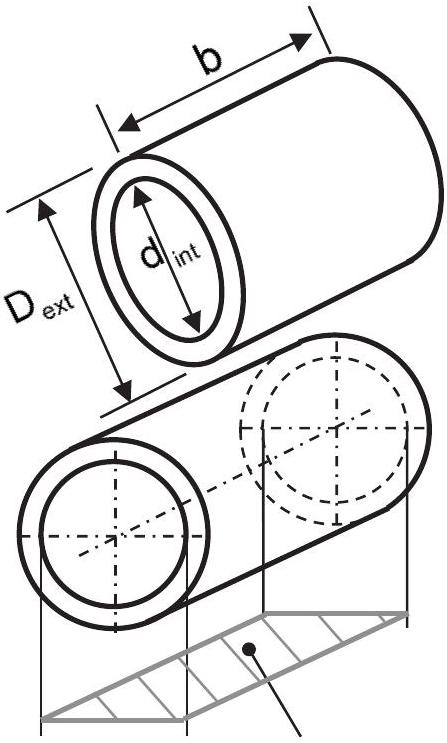
\includegraphics[alt={},max width=\textwidth]{076c1ba0-5a37-41d5-876a-83fc91dd5c32-16_743_447_1638_1458}
\captionsetup{labelformat=empty}
\caption{Surface projetée}
\end{center}
\end{figure}

La force de fermeture du moule de la presse à injecter étudiée vaut $F=1000 k N$. Cet effort statique permet de s'opposer à l'ouverture du moule sous l'effet de l'injection sous forte pression du plastique ramolli. Cet effort F est supporté par les 4 bielles $\underline{4}$ et est supposé également réparti entre chacune d'elles. La phase étudiée est statique puisque l'injection a lieu lorsque le moule est immobile en position fermée.

Question 29. Préciser l'effort $F_{R}$ que doit supporter chaque coussinet.\\
Question 30. Calculer la pression statique p exercée sur chaque coussinet.\\
Question 31. Sur le critère de pression admissible, vérifier si les coussinets choisis conviennent.

\subsection*{6.2 Vérification de la vitesse de glissement admissible}
On réalise une simulation de fermeture du moule. On suppose que le déplacement en translation du moule se fait selon une loi d'évolution des vitesses en trapèze. On relève l'évolution de la vitesse de rotation $\mathrm{N}_{4 / 5}$ en fonction du temps au niveau d'une des liaisons pivots (figure 13).

\begin{figure}[h]
\begin{center}
  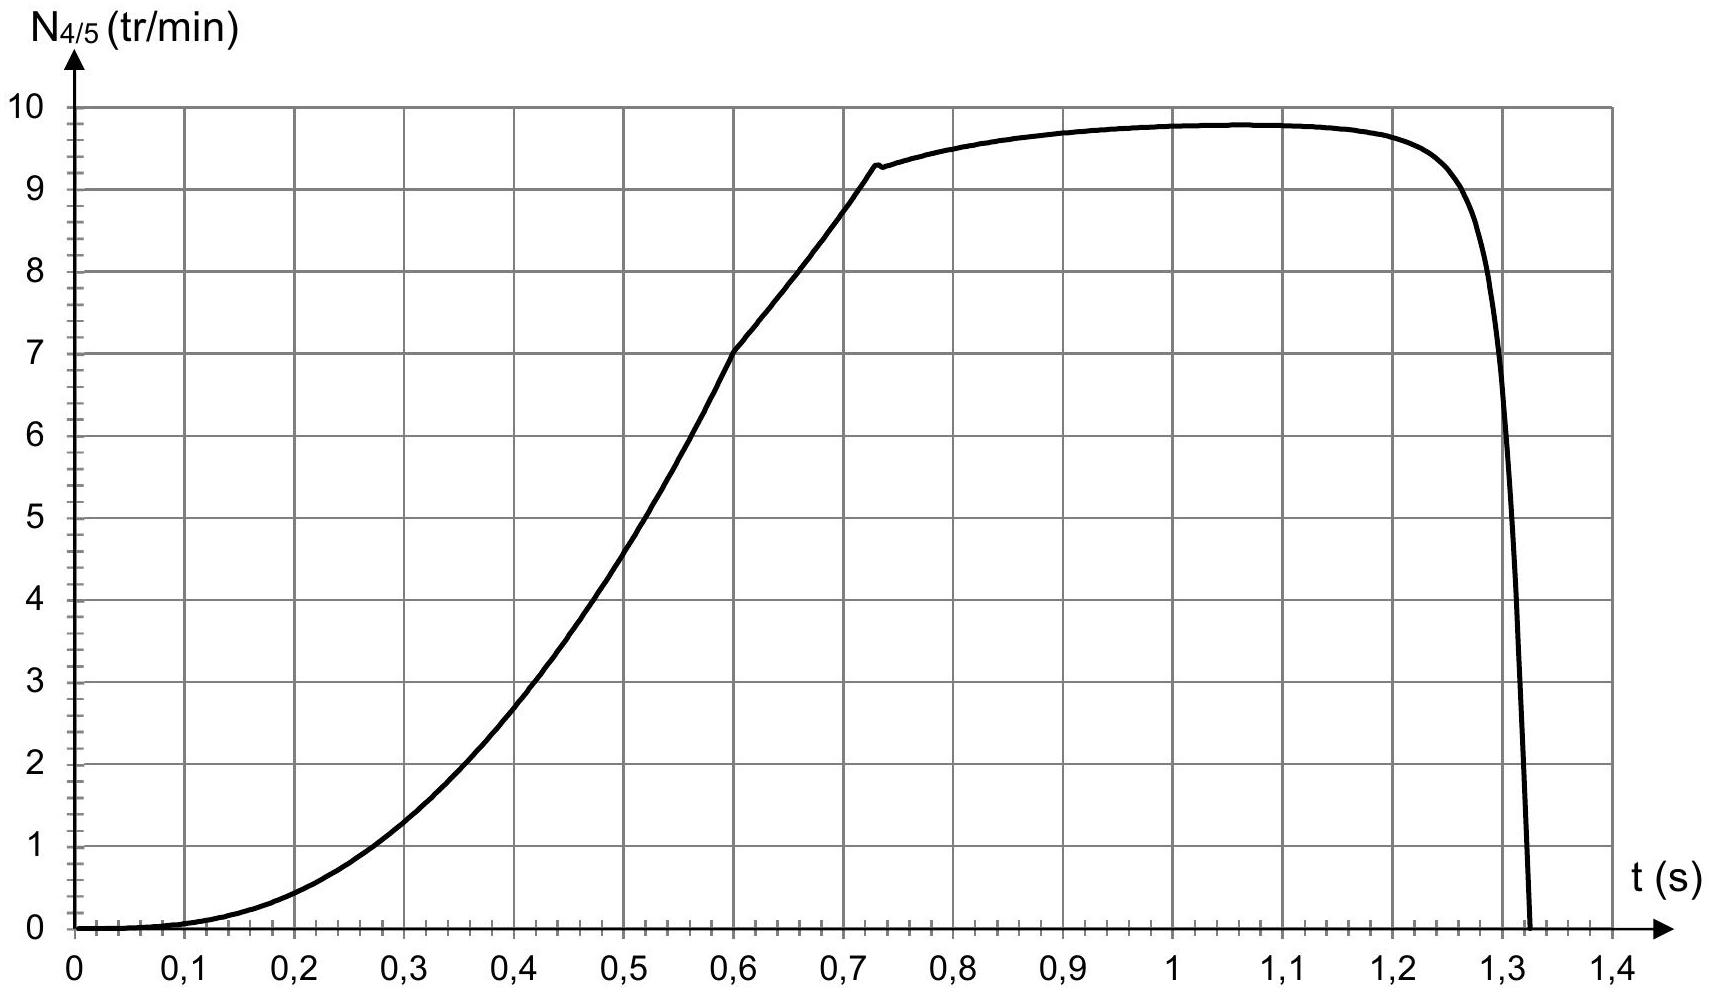
\includegraphics[alt={},max width=\textwidth]{076c1ba0-5a37-41d5-876a-83fc91dd5c32-17_994_1710_868_204}
\captionsetup{labelformat=empty}
\caption{Figure 13 : Norme de la vitesse de rotation $\mathrm{N}_{4 / 5}$ lors d'une fermeture de moule}
\end{center}
\end{figure}

Question 32. Exprimer la vitesse de glissement $\mathrm{v}_{\text {gliss }}$ au niveau des coussinets en fonction de $\mathrm{N}_{4 / 5}$ et $\mathrm{d}_{\text {int }}$.

Question 33. Relever la valeur maximale de $\mathrm{N}_{4 / 5}$ sur la figure 13. En déduire la valeur maximale de la vitesse de glissement et vérifier si les coussinets choisis conviennent.

\section*{PARTIE 7. ASSERVISSEMENT EN TEMPERATURE DU FOURREAU}
Objectifs : Modéliser l'ensemble fourreau/vis, régler le correcteur de l'asservissement en température et vérifier les performances de l'ensemble relatives aux exigences "111", "141" et "142".

Lors de l'injection, la température de la matière est capitale, car si elle est trop froide la matière risque de ne pas être suffisamment fluide pour remplir correctement le moule. À l'inverse, une matière injectée trop chaude risque de ne pas avoir les propriétés plastiques attendues en refroidissant. Il est donc important de chauffer l'ensemble fourreau et vis avec un asservissement précis pour garantir une bonne injection dans le moule.

\subsection*{7.1. Modélisation de l'ensemble Fourreau et vis}
Le fourreau et la vis sont chauffés par le biais de colliers chauffants installés autour du fourreau. Plusieurs sondes de température assurent la surveillance et la mesure de la température dans le fourreau. Un isolant thermique est installé autour de l'ensemble. On retrouve cet ensemble en figure 14.

\begin{figure}[h]
\begin{center}
  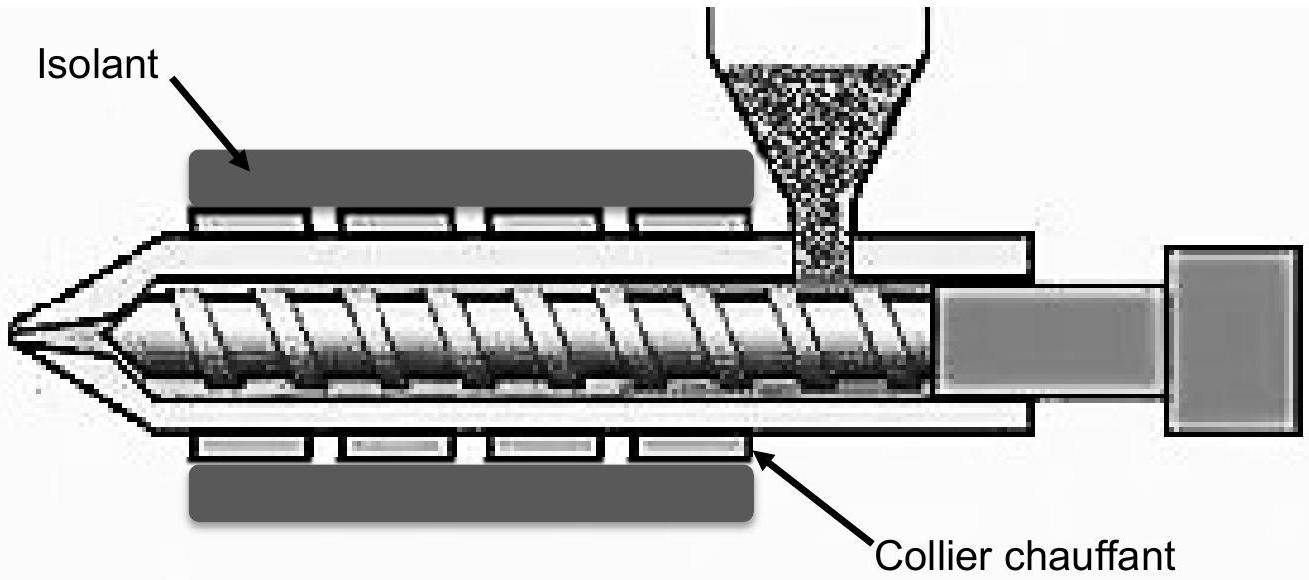
\includegraphics[alt={},max width=\textwidth]{076c1ba0-5a37-41d5-876a-83fc91dd5c32-18_580_1309_1128_370}
\captionsetup{labelformat=empty}
\caption{Figure 14 : Ensemble fourreau, vis, collier chauffant et isolant}
\end{center}
\end{figure}

Afin de modéliser le comportement thermique de cet ensemble, on utilise une analogie possible avec un circuit électrique. L'ensemble fourreau/vis est modélisé par un condensateur analogue à une capacité thermique qui va accumuler de la chaleur. On néglige ici l'influence de la matière plastique. L'isolant est modélisé par une résistance analogue à la résistance thermique qui va limiter l'échange de chaleur entre l'ensemble fourreau/vis et l'air ambiant. Les colliers chauffants sont eux modélisés par une source de courant analogue à une source de puissance thermique.

Dans cette modélisation, le potentiel électrique est analogue à la température d'un élément et le courant à une puissance thermique circulant entre les différents éléments.

Avec des hypothèses simplificatrices sur les effets de bords (correspondant à chaque extrémité du fourreau), en ne considérant que les échanges thermiques par conduction dans l'isolant et en faisant une équivalence de l'ensemble, les dimensions et caractéristiques de cet ensemble donnent le modèle équivalent en figure 15.

\begin{figure}[h]
\begin{center}
  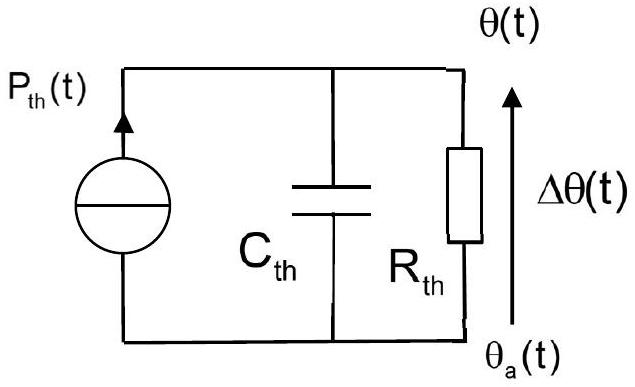
\includegraphics[alt={},max width=\textwidth]{076c1ba0-5a37-41d5-876a-83fc91dd5c32-19_387_635_318_678}
\captionsetup{labelformat=empty}
\caption{Figure 15 : Modèle équivalent thermique de l'ensemble}
\end{center}
\end{figure}

$\mathrm{P}_{\mathrm{th}}(\mathrm{t})$ est la puissance thermique des colliers en Watts.\\
La puissance maximale des colliers chauffants est de 30 kW\\
$\mathrm{C}_{\mathrm{th}}$ est la capacité thermique de l'ensemble en Joule par Kelvin : $\mathrm{C}_{\mathrm{th}}=158.10^{3} \mathrm{JK}^{-1}$\\
$R_{t h}$ est la résistance thermique de l'isolant en Kelvin par Watts: $R_{t h}=17,56.10^{-3} \mathrm{~K} . \mathrm{W}^{-1}$\\
Question 34. Montrer que l'équation différentielle entre $\Delta \theta(\mathrm{t})$ et $\mathrm{P}_{\mathrm{th}}(\mathrm{t})$ est la suivante :

$$
P_{t h}(t)=\frac{\Delta \theta(t)}{R_{t h}}+C_{t h} \frac{d \Delta \theta(t)}{d t}
$$

Question 35. Dans les conditions de Heaviside, écrire cette équation dans le domaine symbolique de Laplace et montrer que la fonction de transfert $\mathrm{H}(\mathrm{p})$ telle que $\Delta \theta(p)=H(p) \times P_{t \mathrm{th}}(p)$ est donnée par :

$$
H(p)=R_{t h} \frac{1}{1+R_{t h} C_{t h} p}
$$

Question 36. Quel est l'ordre et la classe de cette fonction de transfert?\\
La transformée de Laplace d'une constante étant nulle, on montre que la fonction de transfert entre $\theta(p)$ et $P_{\text {th }}(p)$ est $H(p)$. Ainsi $\theta(p)=H(p) \times P_{\text {th }}(p)$ où $\theta(p)$ peut être exprimé indifféremment en Kelvin ou en degré.

\subsection*{7.2. Asservissement avec correcteur proportionnel}
On asservit la température avec un correcteur de type proportionnel de valeur $\mathrm{K}_{\mathrm{p}}$. Le modèle de la boucle d'asservissement dans le domaine symbolique de Laplace est donné figure 16.

\begin{figure}[h]
\begin{center}
  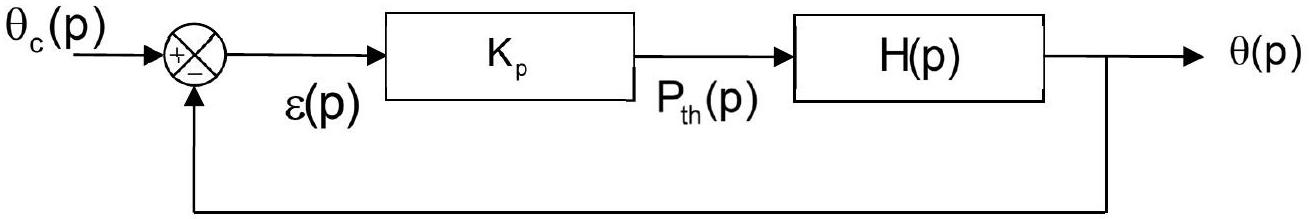
\includegraphics[alt={},max width=\textwidth]{076c1ba0-5a37-41d5-876a-83fc91dd5c32-19_219_1309_2259_380}
\captionsetup{labelformat=empty}
\caption{Figure 16 : Boucle d'asservissement avec correcteur proportionnel}
\end{center}
\end{figure}

Question 37. Déterminer la fonction de transfert en boucle fermée $\mathrm{FTBF}_{1}(\mathrm{p})$ et donner les caractéristiques de cette fonction de transfert.

Question 38. Le système ainsi asservi présente-t-il un problème de stabilité ? Justifier.\\
Question 39. Déterminer l'expression de $\varepsilon(\mathrm{p})$ en fonction de $\theta_{\mathrm{c}}(\mathrm{p})$ et des fonctions de transfert de la boucle d'asservissement.

On soumet ce système à une consigne de température $\theta_{\mathrm{c}}(\mathrm{t})$ du type échelon telle que $\theta_{\mathrm{c}}(\mathrm{p})=\frac{\theta_{\mathrm{c}}}{\mathrm{p}}$.\\
Question 40. Déterminer l'erreur statique relative de cet asservissement en réponse à cette sollicitation. Donner un critère permettant d'obtenir une erreur statique relative inférieure à 0,1\% pour satisfaire l'exigence "142".

Question 41. Compte tenu des expressions de la $\mathrm{FTBF}_{1}(\mathrm{p})$ et de l'erreur statique relative, que doit-on faire pour améliorer l'erreur statique et la dynamique du système ?

Question 42. Quel type de correcteur permettrait d'annuler l'erreur statique indépendamment des variations du correcteur proportionnel ?

Sans changer la nature du correcteur, on prendra pour la suite $K_{p}=60000$.\\
Question 43. Déterminer en conséquence la constante de temps caractéristique de la $\mathrm{FTBF}_{1}(\mathrm{p})$ ainsi le temps de réponse à 5\% du système bouclé, conclure vis-à-vis de l'exigence "141".

Question 44. Déterminer l'expression de $\mathrm{P}_{\mathrm{th}}(\mathrm{p})$ en fonction de $\theta_{\mathrm{c}}(\mathrm{p})$ et des fonctions de transfert de la boucle d'asservissement.

Question 45. En déduire la valeur de $\mathrm{P}_{\text {th }}(\mathrm{t})$ au démarrage du système pour une augmentation de la température dans le fourreau de $220^{\circ} \mathrm{C}$ correspondant à $\quad \theta_{\mathrm{c}}(\mathrm{p})=\frac{220}{\mathrm{p}}$.

Question 46. La puissance obtenue étant supérieure à la puissance maximale des colliers chauffants, comment le temps de réponse à 5\% va-t-il être modifié ?

Une simulation sur Matlab Simulink a été réalisée en figure 17.\\
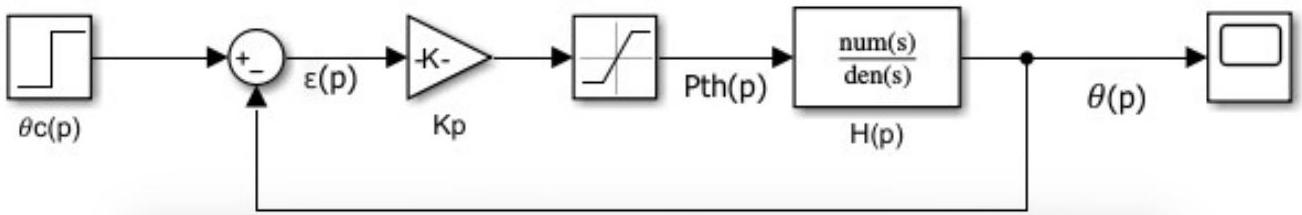
\includegraphics[max width=\textwidth, alt={}, center]{076c1ba0-5a37-41d5-876a-83fc91dd5c32-21_215_1302_379_379}\\

\includegraphics[max width=\textwidth, alt={}, center]{076c1ba0-5a37-41d5-876a-83fc91dd5c32-21_59_1010_617_521}

Saturation\\
Limit input signal to the upper and lower saturation values.\\
Main Signal Attributes\\
Upper limit:\\
v1\\
⋮\\
Lower limit:\\
v2\\
⋮

Treat as gain when linearizing

Enable zero-crossing detection

OK\\
Cancel\\
Help\\
Apply

Question 47. Donner les valeurs de v1 et v2 à régler dans les paramètres du bloc saturation.

\begin{figure}[h]
\begin{center}
\captionsetup{labelformat=empty}
\caption{Figure 17 : Simulation Matlab Simulink de l'asservissement de température}
  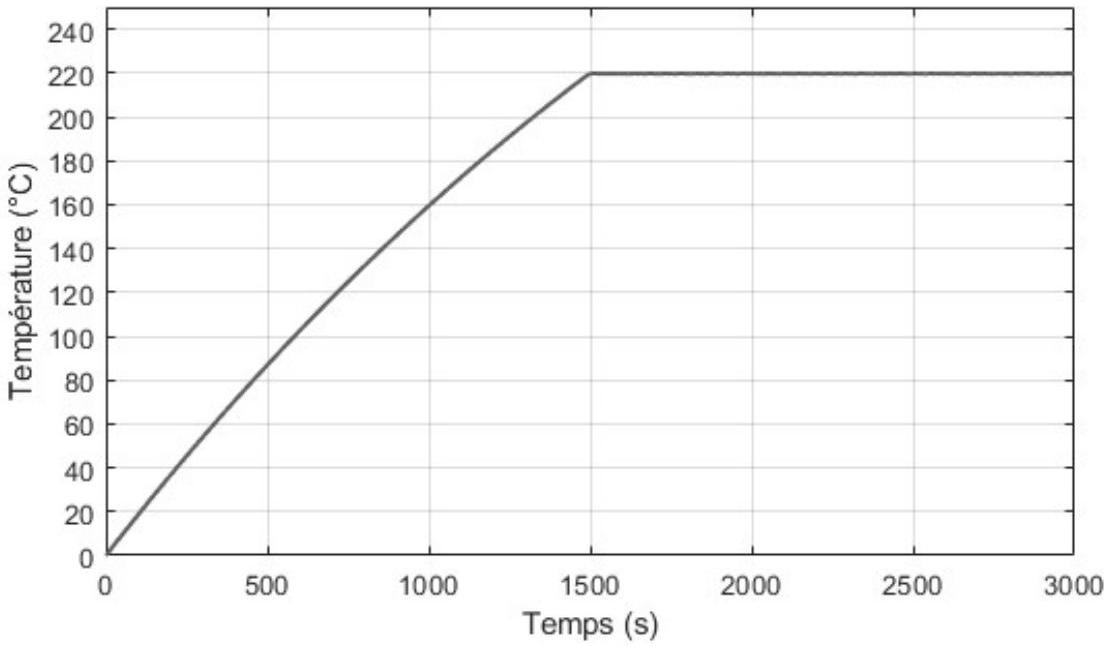
\includegraphics[alt={},max width=\textwidth]{076c1ba0-5a37-41d5-876a-83fc91dd5c32-21_646_1112_1674_464}
\end{center}
\end{figure}

Figure 18 : Résultat de la simulation Matlab Simulink de l'asservissement de température

Question 48. À partir du résultat de la simulation en figure 18, mesurer le temps de réponse à 5\%. Comparer ce temps avec la valeur calculée à la question 43. Expliquer cet écart. Conclure quant au respect de l'exigence "111".

\section*{PARTIE 8. ALIMENTATION DE LA MACHINE D'ENTRAINEMENT DE LA VIS DU FOURREAU}
Objectif : Etudier l'ensemble d'alimentation de la machine d'entraînement de la vis du fourreau et valider l'exigence "13".

La rotation de la vis du fourreau a deux rôles. Le premier est de mélanger les granulats de plastique entrant dans le fourreau par l'entonnoir. Avec la chaleur, les granulats vont fondre et la matière ainsi malaxée va s'homogénéiser. Le deuxième rôle de la rotation est de faire avancer la matière plastique fondue à l'extrémité de la vis. Cette matière passera par un clapet anti-retour en bout de vis. Ainsi la vis recule tout en tournant. C'est la phase de dosage.

L'entraînement en rotation de la vis du fourreau est assuré par une machine asynchrone par le biais d'un réducteur de vitesse. La variation de vitesse de la vis du fourreau n'est pas nécessaire, en conséquence, l'alimentation électrique de la machine asynchrone est composée d'un redresseur monophasé, d'un filtre et d'un onduleur pleine onde. La structure globale de l'alimentation électrique est donnée figure 19.

\begin{figure}[h]
\begin{center}
  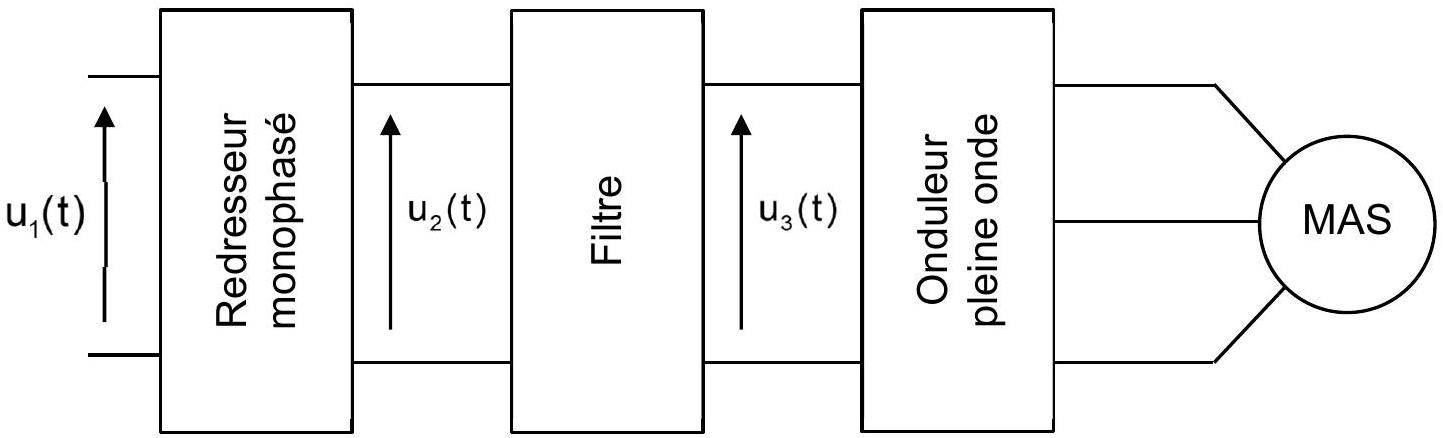
\includegraphics[alt={},max width=\textwidth]{076c1ba0-5a37-41d5-876a-83fc91dd5c32-22_438_1443_1087_310}
\captionsetup{labelformat=empty}
\caption{Figure 19 : Structure globale de l'alimentation électrique}
\end{center}
\end{figure}

\subsection*{8.1. Redresseur monophasé et filtre}
Le redresseur monophasé est composé d'un pont de diodes. On considère ici que le filtre n'a pas d'influence sur la forme d'onde en sortie du pont de diodes.

\begin{figure}[h]
\begin{center}
  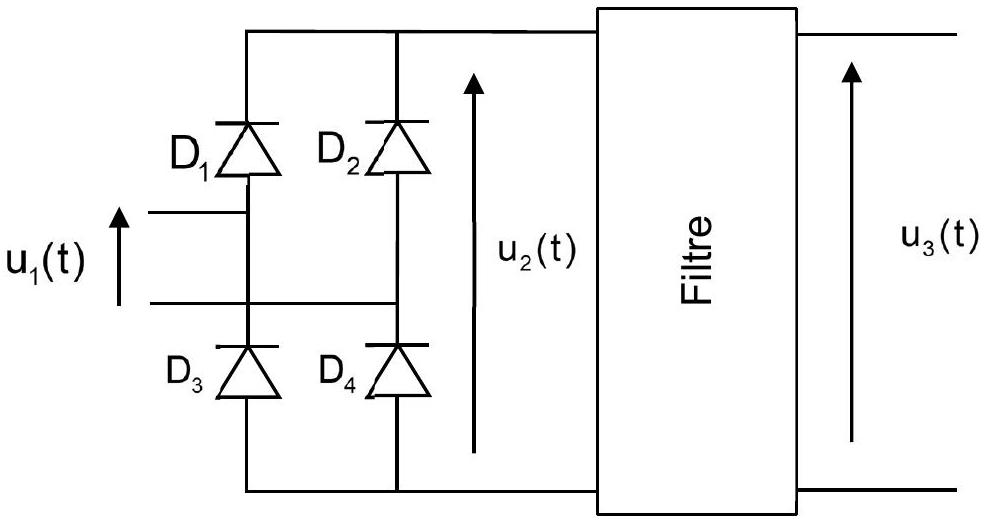
\includegraphics[alt={},max width=\textwidth]{076c1ba0-5a37-41d5-876a-83fc91dd5c32-22_520_989_1835_532}
\captionsetup{labelformat=empty}
\caption{Figure 20 : Pont de diodes et filtre}
\end{center}
\end{figure}

Question 49. À partir de la figure 20, compléter le document réponse 1 en indiquant pour chaque courbe la tension du montage correspondante.

Question 50. De quel type de convertisseur s'agit-il ?

\subsection*{8.2. Onduleur pleine onde}
La machine qui entraîne la vis en rotation est une machine asynchrone triphasée. En conséquence, on utilise un onduleur triphasé pour alimenter cette machine à partir de la tension $\mathrm{u}_{3}(\mathrm{t})$ considérée quasi constante de valeur $E=200 V$. En considérant les commutateurs statiques parfaits équivalents à des interrupteurs, le schéma électrique de l'onduleur est donné figure 21. La loi de commande de type plein onde de cet onduleur est donnée sur le document réponse 2.

\begin{figure}[h]
\begin{center}
  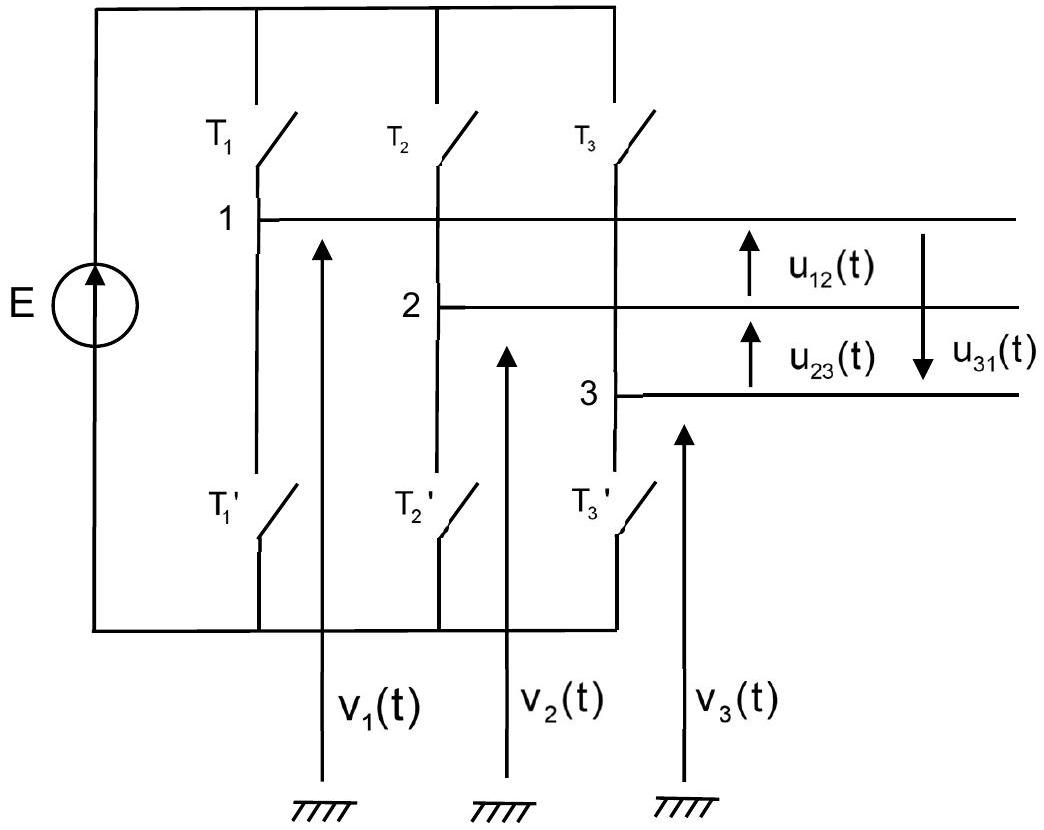
\includegraphics[alt={},max width=\textwidth]{076c1ba0-5a37-41d5-876a-83fc91dd5c32-23_830_1044_657_464}
\captionsetup{labelformat=empty}
\caption{Figure 21 : Onduleur triphasé pleine onde}
\end{center}
\end{figure}

Question 51. Justifier que, pour chaque bras d'onduleur, les interrupteurs $T_{x}$ et $T_{x}{ }^{\prime}$ ne peuvent pas être fermés simultanément.

Question 52. Donner les valeurs des tensions $\mathrm{u}_{12}(\mathrm{t}), \mathrm{u}_{23}(\mathrm{t})$ et $\mathrm{u}_{31}(\mathrm{t})$ à tout instant sur le document réponse 2.

La loi de commande et la machine étant équilibrée, on en déduit que

$$
\mathrm{v}_{1}(\mathrm{t})+\mathrm{v}_{2}(\mathrm{t})+\mathrm{v}_{3}(\mathrm{t})=0 \quad \text { et } \quad \mathrm{u}_{12}(\mathrm{t})+\mathrm{u}_{23}(\mathrm{t})+\mathrm{u}_{31}(\mathrm{t})=0 .
$$

Question 53. Montrer que :

\begin{itemize}
  \item[-] $\mathrm{v}_{1}(\mathrm{t})=1 / 3\left(\mathrm{u}_{12}(\mathrm{t})-\mathrm{u}_{31}(\mathrm{t})\right)$
  \item[-] $\mathrm{v}_{2}(\mathrm{t})=1 / 3\left(\mathrm{u}_{23}(\mathrm{t})-\mathrm{u}_{12}(\mathrm{t})\right)$
  \item[-] $\mathrm{v}_{3}(\mathrm{t})=1 / 3\left(\mathrm{u}_{31}(\mathrm{t})-\mathrm{u}_{23}(\mathrm{t})\right)$
\end{itemize}

Question 54. Donner les valeurs des tensions $\mathrm{v}_{1}(\mathrm{t}), \mathrm{v}_{2}(\mathrm{t})$ et $\mathrm{v}_{3}(\mathrm{t})$ à tout instant et tracer leurs allures sur le document réponse 3.

\section*{PARTIE 9. PROTOCOLE DE COMMUNICATION MODULE MOTEUR ET CAPTEUR DU ROBOT DE DECHARGEMENT}
Objectif : Etudier le protocole de transmission entre le robot et la machine à injection et vérifier l'exigence "152" relative à la précision minimale que doit avoir le robot.

Le robot de déchargement est un robot de type cartésien 3 axes. Le constructeur a choisi une configuration modulable qui permet de choisir le nombre d'axes du robot (figure 22).\\
Chaque axe est donc composé d'un ensemble mécanique permettant la translation, d'un motoréducteur, d'un capteur linéaire de type incrémental et d'un module de puissance. Une centrale de gestion permet le contrôle du motoréducteur et la communication de l'ensemble.

\begin{figure}[h]
\begin{center}
  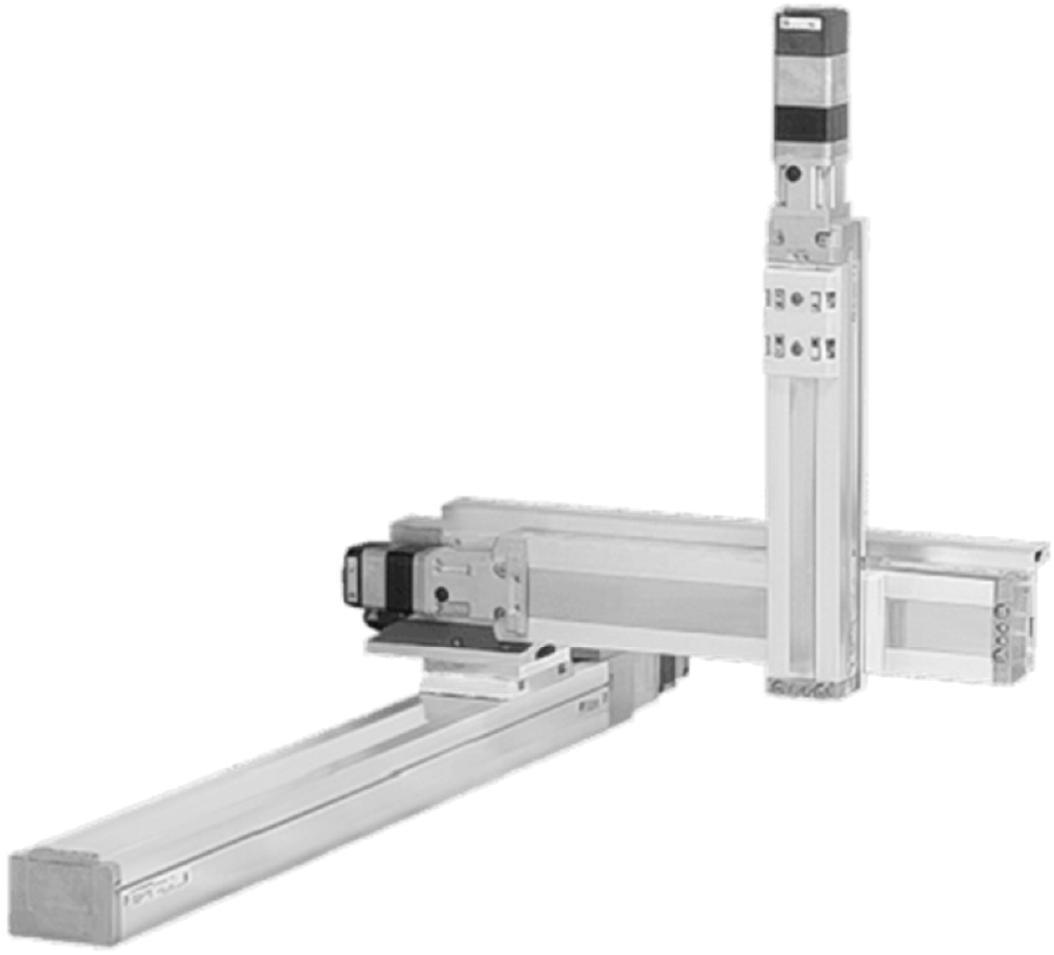
\includegraphics[alt={},max width=\textwidth]{076c1ba0-5a37-41d5-876a-83fc91dd5c32-24_955_1054_888_440}
\captionsetup{labelformat=empty}
\caption{Figure 22 : Robot cartésien 3 axes}
\end{center}
\end{figure}

La centrale de gestion récupère les informations de position des axes du capteur linéaire par le biais de l'interface de communication. Elle commande en retour les modules de puissance en passant par cette même interface de communication.\\
Conformément à l'exigence "151", un protocole « full-duplex » est utilisé, ici le RS232.\\
Quelques éléments du protocole RS232 sont détaillés en annexe 5.\\
Question 55. En quoi consiste un protocole « full-duplex » ?\\
Question 56. Le protocole RS232 est dit asynchrone. Expliquer ce terme. En déduire l'intérêt du bit de start. En conséquence, quel réglage préalable est-il nécessaire d'effectuer sur la centrale de gestion et un module d'axe ?

Question 57. Expliquer le principe de fonctionnement du bit de parité. Quelle est son utilité ? Quelle est sa limitation ?

Le robot cartésien choisi a une course maximale sur chaque axe de 1500 mm. La position linéaire issue du capteur incrémental est une valeur numérique codée sur 16 bits.

Question 58. Combien de trames seront nécessaires pour transmettre une information de position à la centrale de gestion ?

Question 59. Quelle est la plus petite variation de déplacement du robot détectable par le capteur linéaire ? Conclure vis-à-vis de l'exigence "152".

Une mesure du signal émise par un module d'axe à la centrale de gestion est affichée figure 23.

\begin{figure}[h]
\begin{center}
  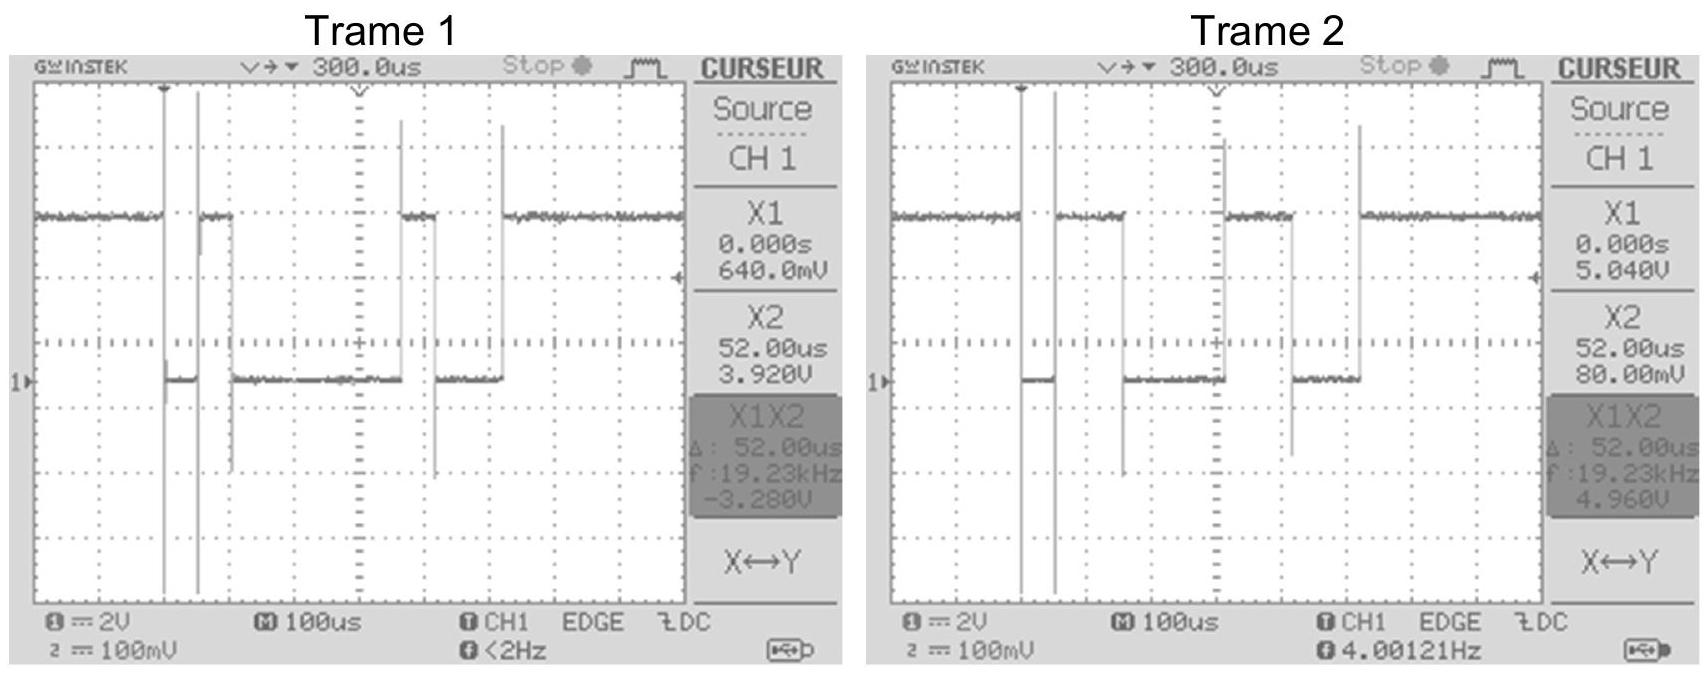
\includegraphics[alt={},max width=\textwidth]{076c1ba0-5a37-41d5-876a-83fc91dd5c32-25_674_1706_741_178}
\captionsetup{labelformat=empty}
\caption{Figure 23 : Trames séries émises par un module d'axe}
\end{center}
\end{figure}

Les données sont envoyées en commençant par les bits de poids faible.\\
Question 60. Mesurer la durée d'envoi d'un bit, en déduire le débit binaire de la transmission.\\
Question 61. Identifier les deux octets transmis et recomposer le nombre binaire correspondant à la position transmise, donner la valeur décimale correspondante.

Question 62. En déduire la position linéaire de l'axe à partir des questions 58 et 60.\\
Question 63. Sachant que l'on peut enchaîner les transmissions d'octets par un bit de start dès la fin des 2 bits de stop, quelle est la durée minimale pour transmettre une information de position ?

Afin de stopper la production et avertir l'opérateur d'un dysfonctionnement, des trames d'alarme doivent être envoyées par le robot à la machine à injection.\\
Pour ne pas entrer en contact avec le moule ou des éléments structurels de la machine, le robot doit limiter ses mouvements sur une plage pour chacun de ses 3 axes.\\
Pour l'axe $\vec{x}_{0}$, les mouvements doivent être limités entre 375 mm et 750 mm.

Question 64. Recopier et compléter l'algorithme ci-dessous.

\begin{itemize}
  \item[-] La limite\_inf\_x0 est la valeur numérique codée sur 16 bits correspondant à 375 mm
  \item[-] La limite\_sup\_x0 est la valeur numérique codée sur 16 bits correspondant à 750 mm
  \item[-] La fonction lire\_capteur\_x0 renvoie la valeur numérique codée sur 16 bits issue du capteur de l'axe $\overrightarrow{\mathrm{x}}_{0}$.
  \item[-] La fonction allumer\_alarme renvoie un signal permettant de déclencher une alarme
\end{itemize}

--- DEBUT ALGORITHME ---\\
Limite\_inf\_x0 = A COMPLETER\\
Limite\_sup\_x0 = A COMPLETER\\
Valeur = lire\_capteur\_x0\\
(SI ou TANT QUE, utiliser le mot-clé utile) CONDITION A COMPLETER\\
Allumer\_alarme\\
--- FIN ALGORITHME ---

Fin du sujet.

\begin{figure}[h]
\begin{center}
\captionsetup{labelformat=empty}
\caption{req [] Machine à injection plastique [ exigences système ]}
  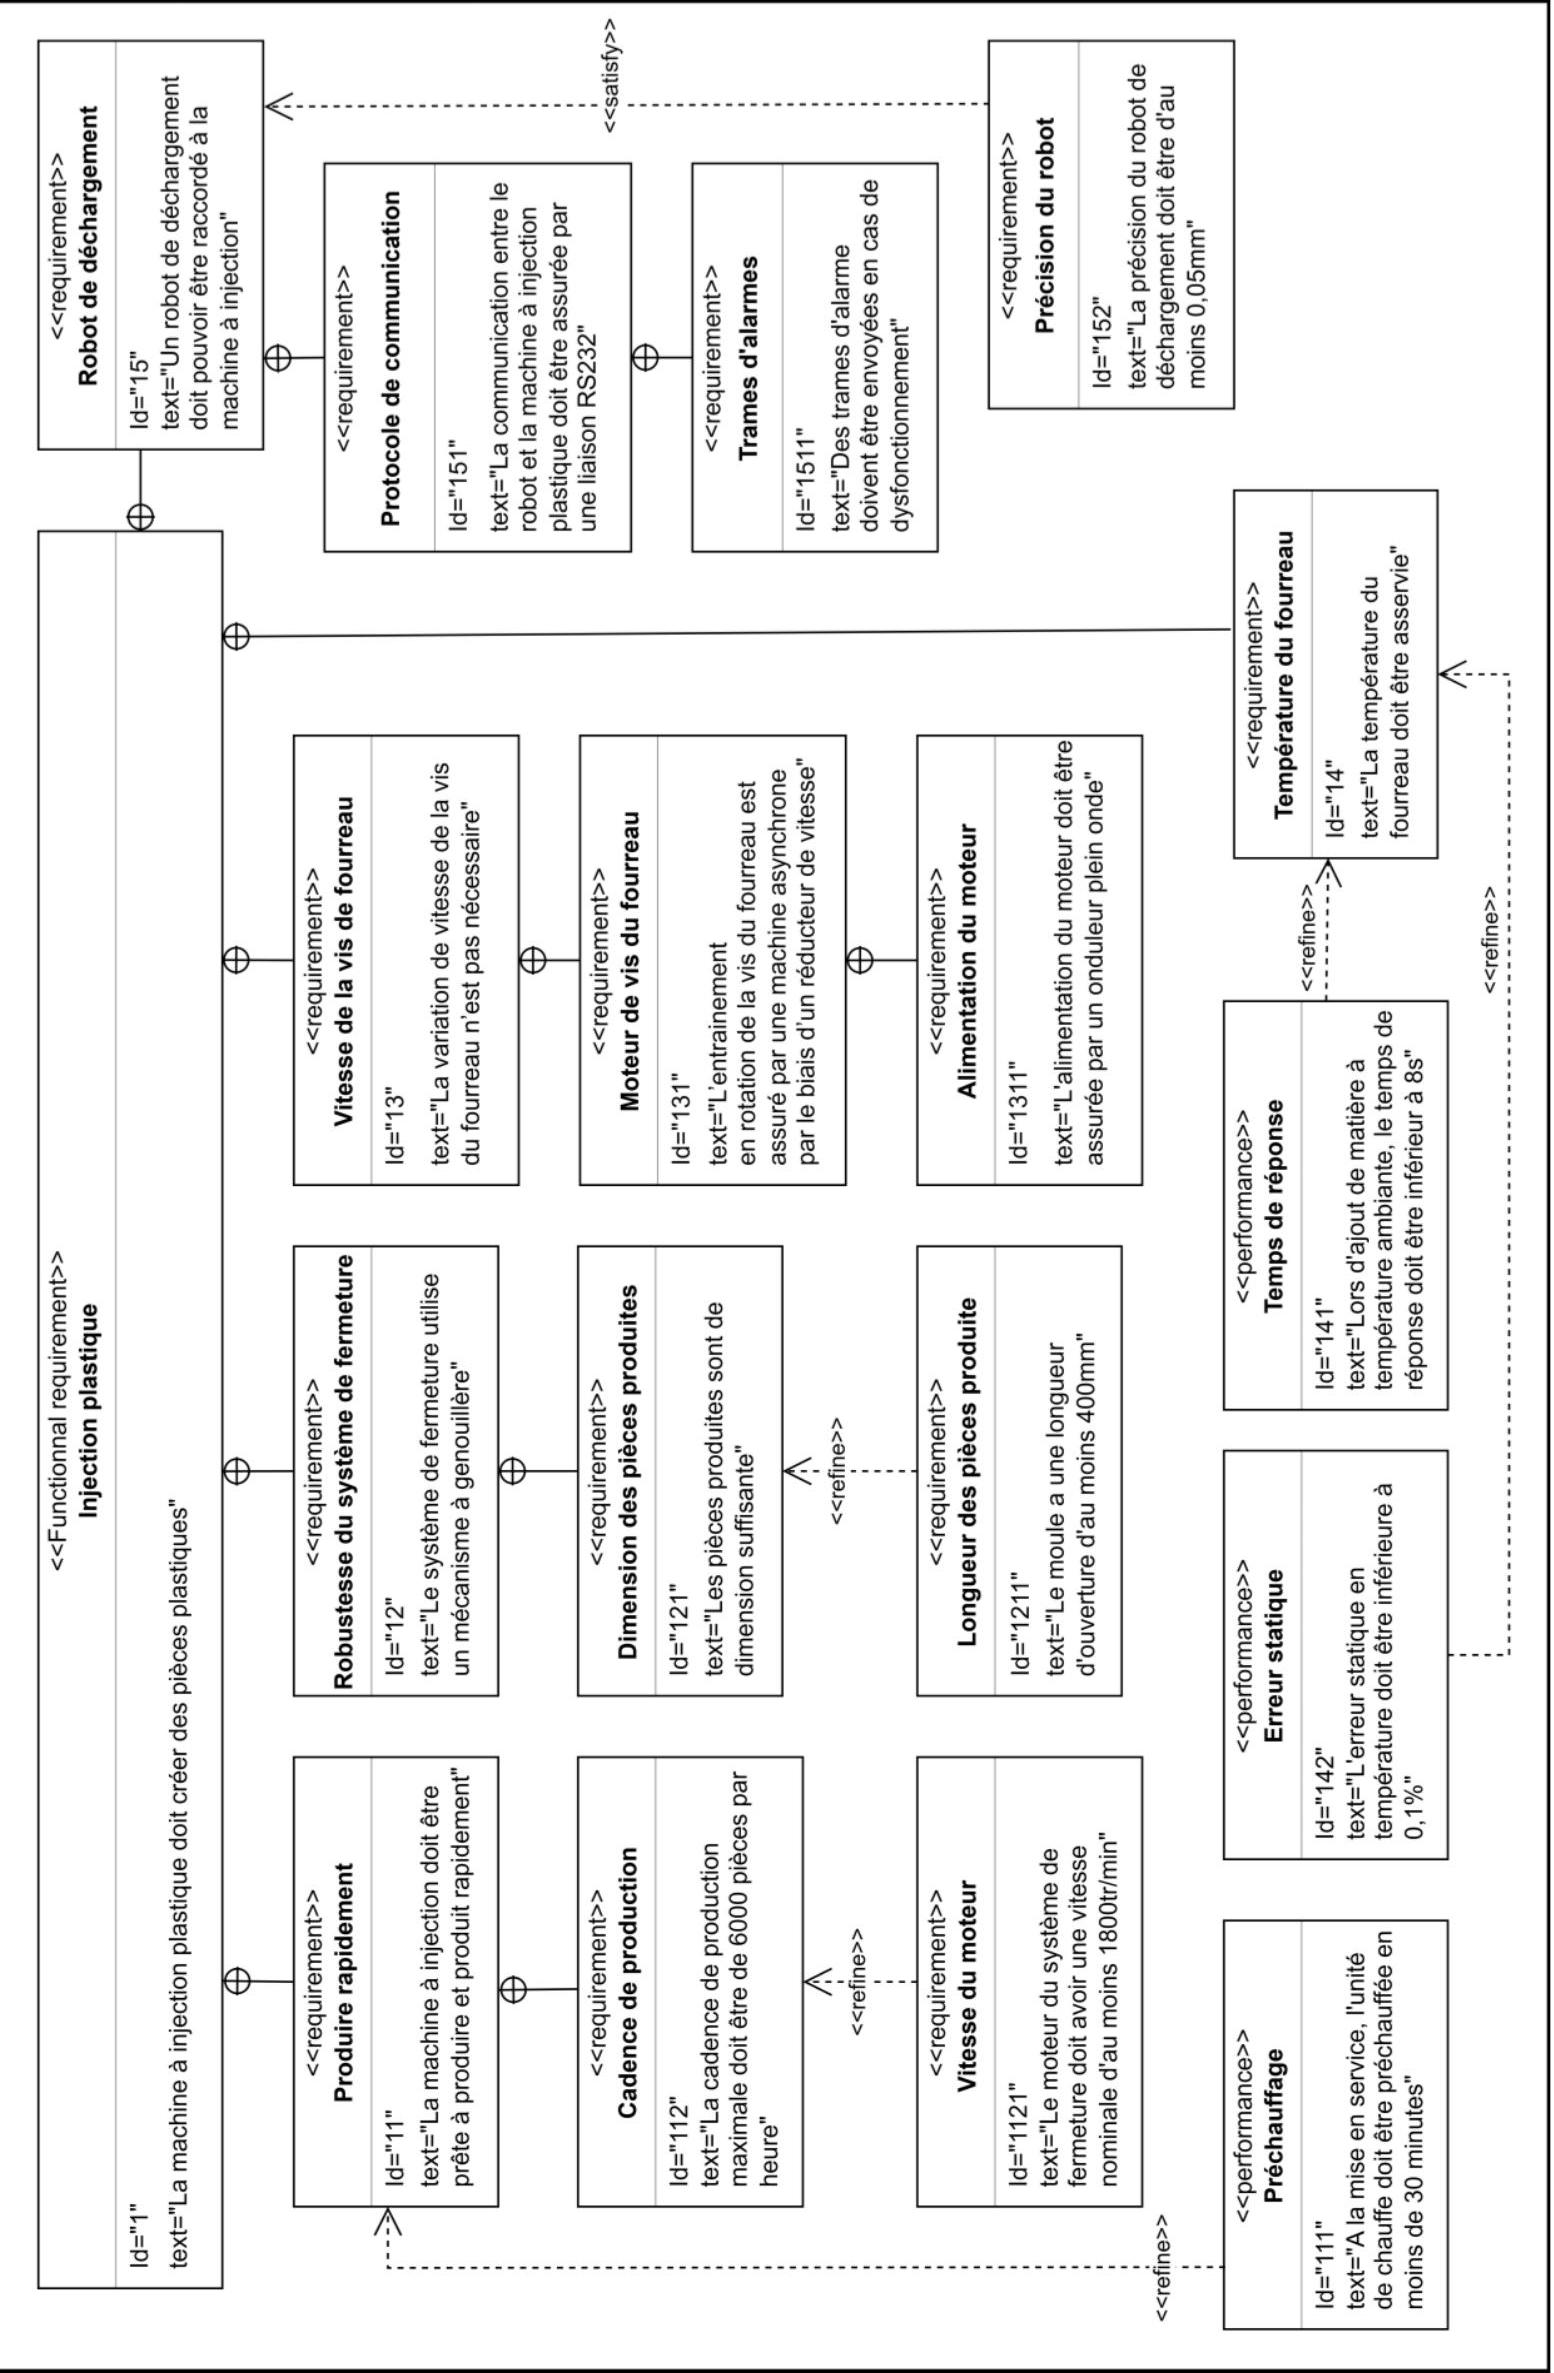
\includegraphics[alt={},max width=\textwidth]{076c1ba0-5a37-41d5-876a-83fc91dd5c32-28_2373_1554_300_280}
\end{center}
\end{figure}

Annexe 2 : schéma cinématique plan complet

\begin{figure}[h]
\begin{center}
  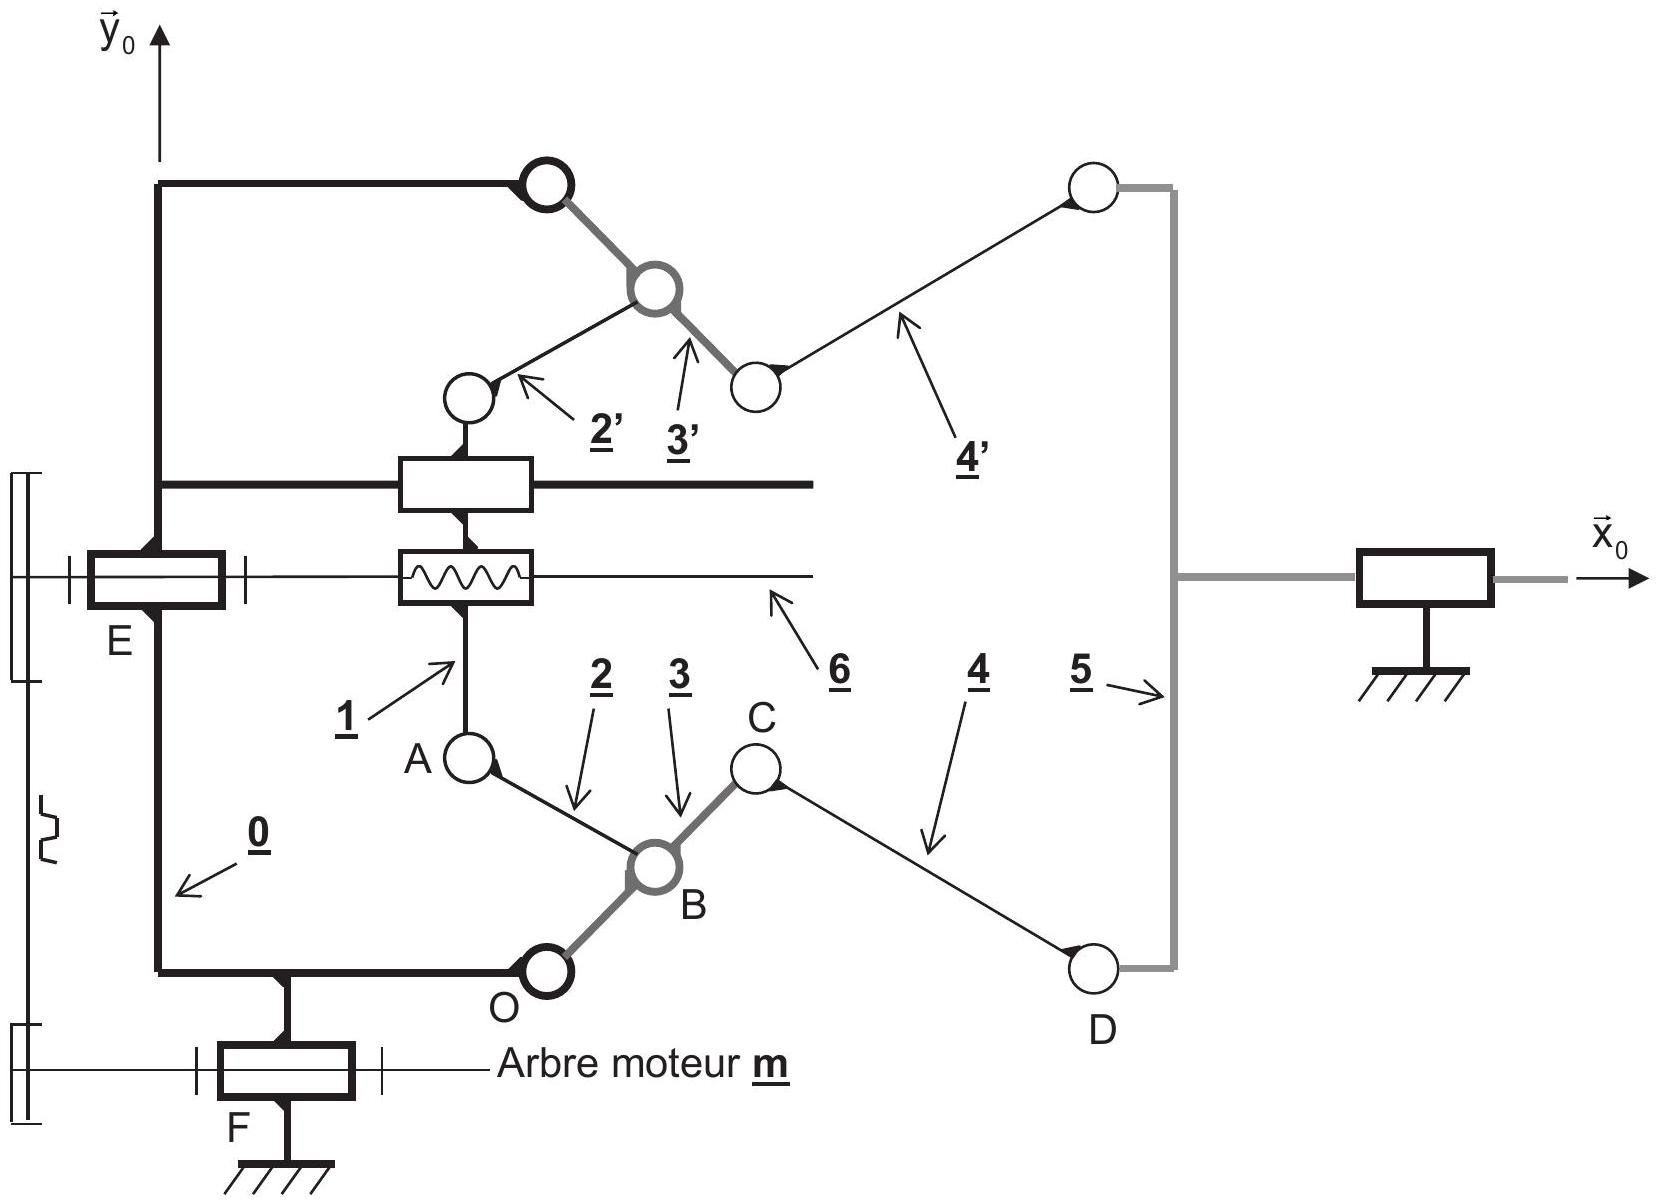
\includegraphics[alt={},max width=\textwidth]{076c1ba0-5a37-41d5-876a-83fc91dd5c32-29_1203_1657_395_185}
\captionsetup{labelformat=empty}
\caption{Schéma cinématique plan, position intermédiaire}
\end{center}
\end{figure}

0 : bâti\\
2 et 2' : biellettes\\
4 et 4' : bielles\\
5 : moule (partie mobile)

1 : écrou\\
$\underline{\mathbf{3}}$ et $\underline{\mathbf{3}}^{\prime}$ : manivelles\\
6 : vis

Transmission par poulies/courroie crantées entre l'arbre moteur $\underline{\mathbf{m}}$ et la vis $\underline{\mathbf{6}}$. Les nombres de dents des poulies sont : $\mathrm{Z}_{\mathrm{m}}=30$ et $\mathrm{Z}_{6}=90$

Pour la liaison hélicoïdale $\underline{\mathbf{6}} / \underline{\mathbf{1}}$, le pas vaut : $\mathrm{p}_{\mathrm{v}}=0,03 \mathrm{~m} / \mathrm{tr}$

Annexe 3 : phases de fonctionnement\\
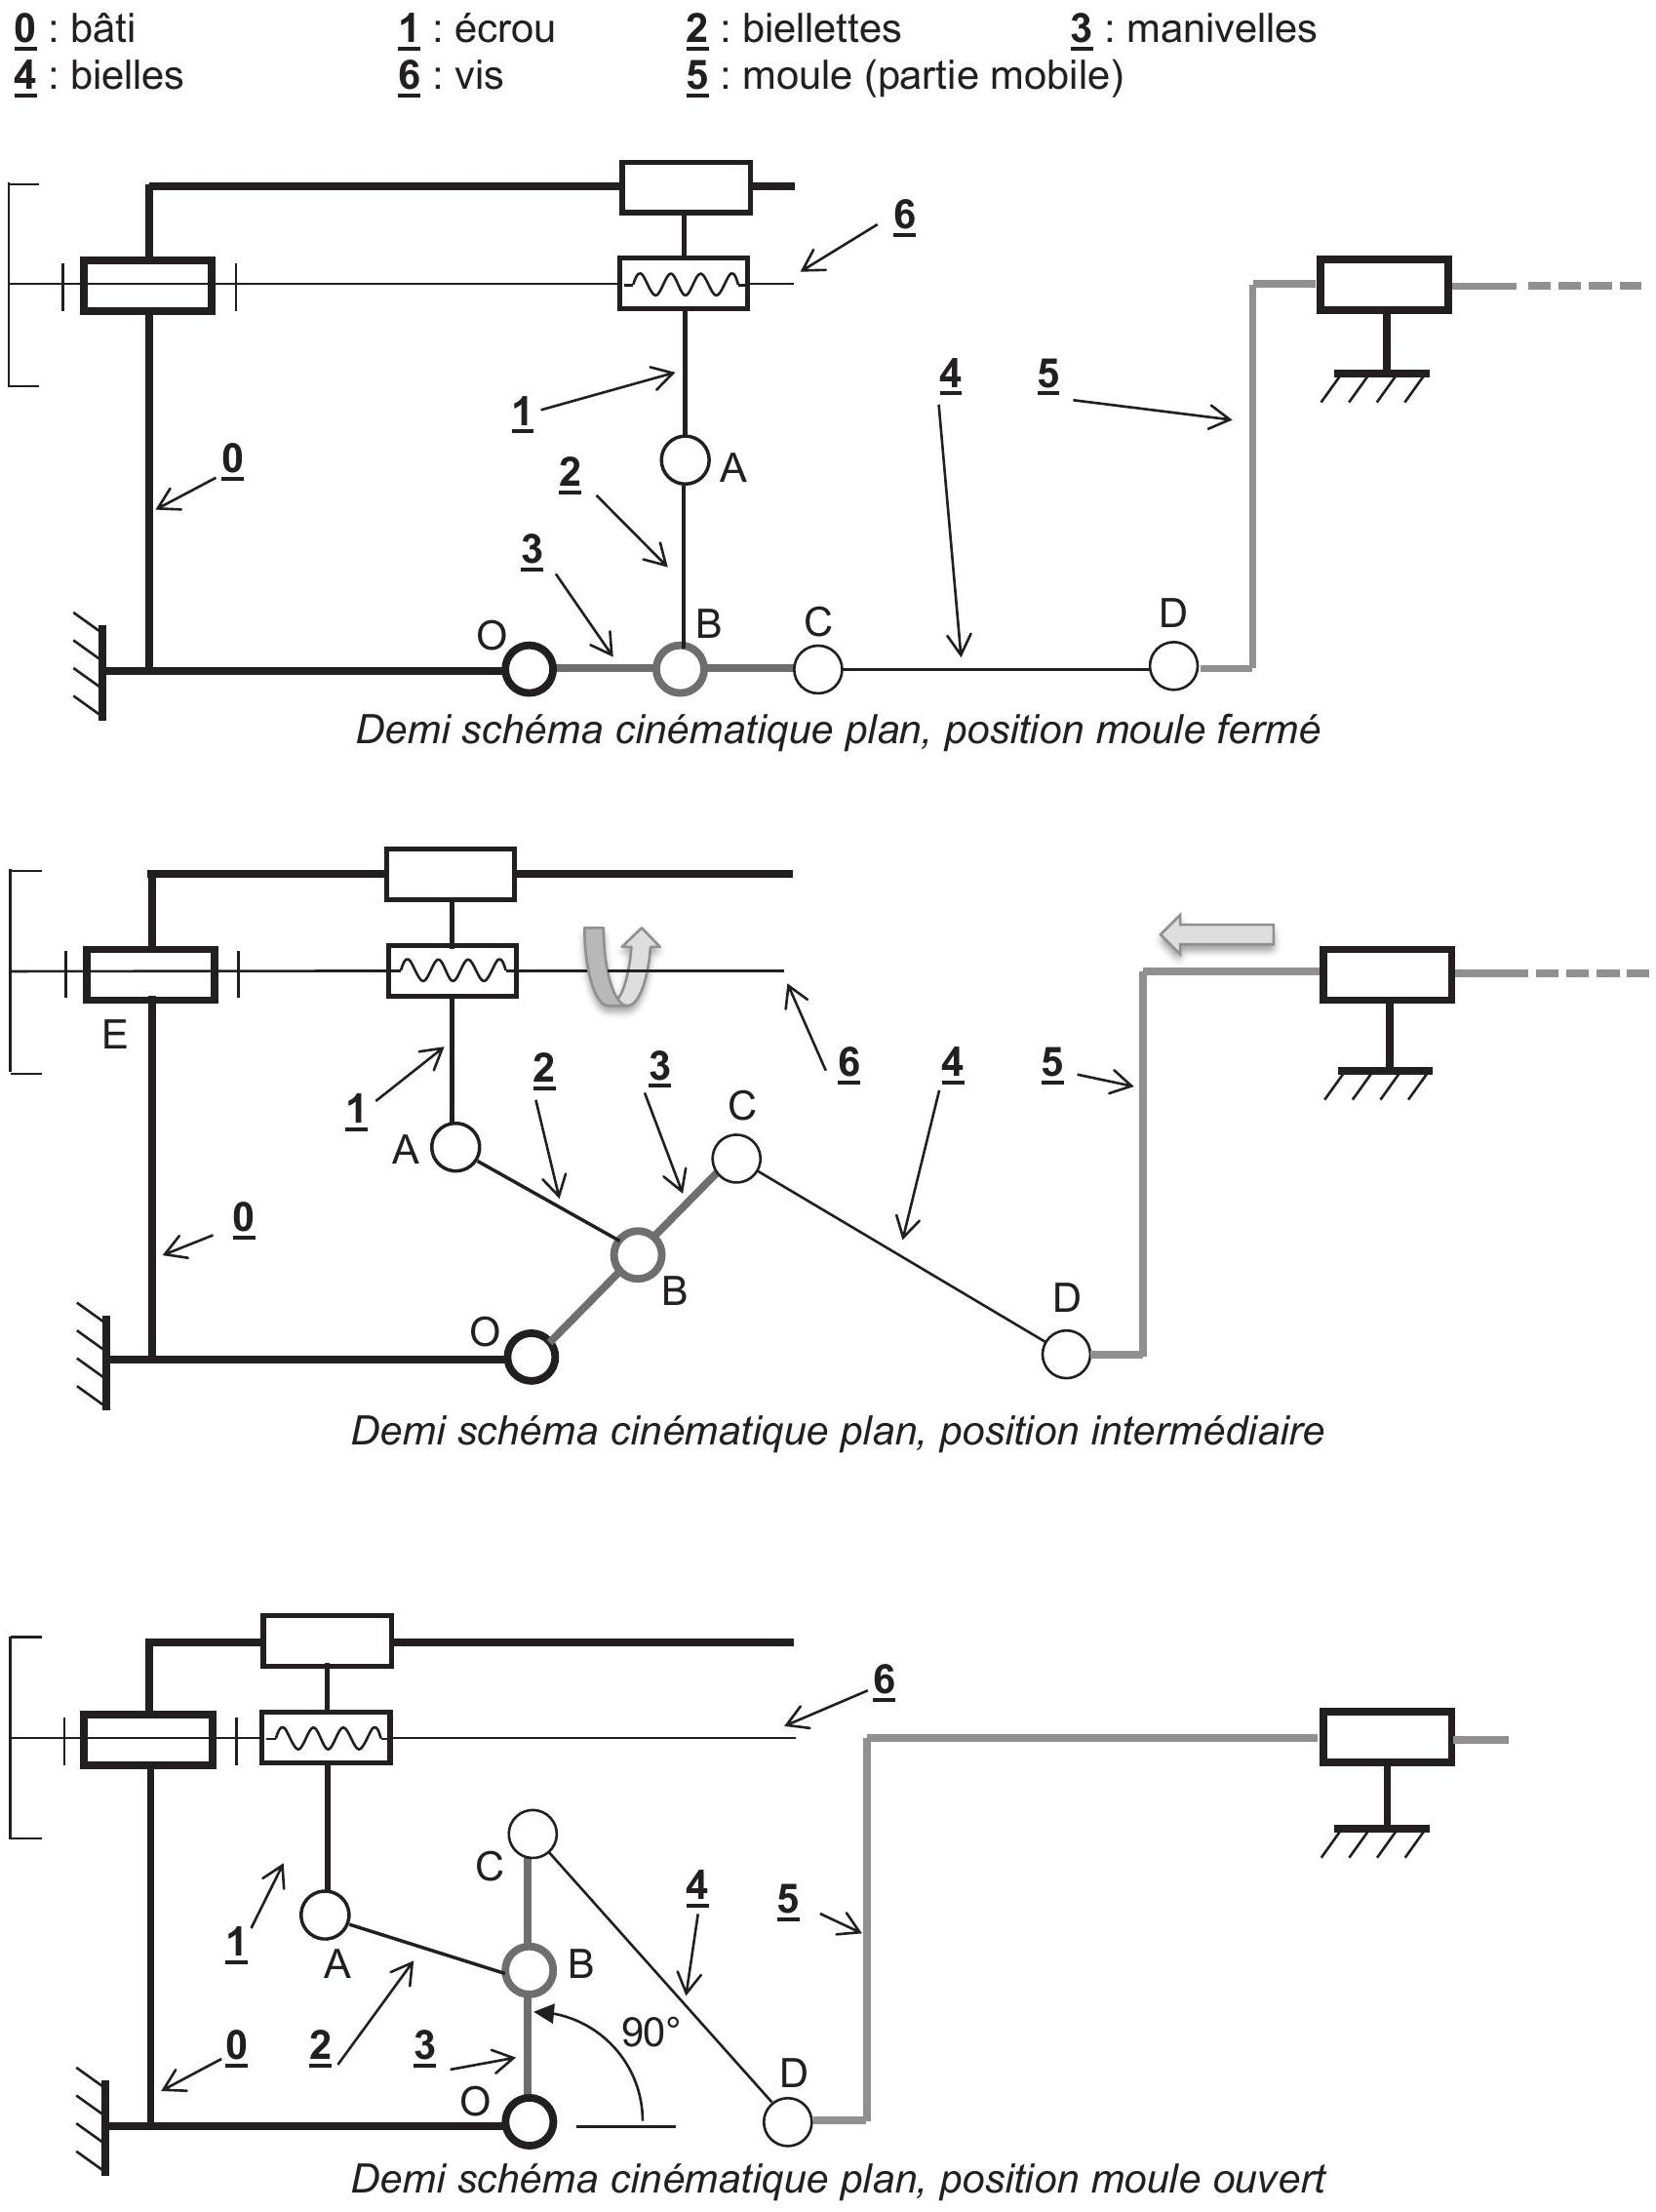
\includegraphics[max width=\textwidth, alt={}, center]{076c1ba0-5a37-41d5-876a-83fc91dd5c32-30_2268_1698_385_173}

\begin{table}[h]
\begin{center}
\captionsetup{labelformat=empty}
\caption{Annexe 4 : documentation moteur électrique}
\begin{tabular}[t]{|l|l|l|l|l|l|l|l|l|l|l|}
\hline
\multirow{2}{*}{Type} & Puissance nominale & Moment nominal & Moment démarrage/ Moment nominal & Moment maximum/ Moment nominal & Intensité démarrage/ Intensité nominale & Moment d'inertie & Masse & Bruit & Vitesse nominale & Intensité nominale \\
\hline
 & $\mathrm{P}_{\mathrm{n}}$ kW & $\mathrm{M}_{\mathrm{n}}$ N.m & $\mathrm{M}_{\mathrm{d}} / \mathrm{M}_{\mathrm{n}}$ & $\mathrm{M}_{\mathrm{m}} / \mathrm{M}_{\mathrm{n}}$ & $\mathrm{I}_{\mathrm{d}} / \mathrm{I}_{\mathrm{n}}$ & J $\mathrm{kg} . \mathrm{m}^{2}$ & IM B3 kg & LP db(A) & $\mathrm{N}_{\mathrm{n}} \mathrm{min}^{-1}$ & $\mathrm{I}_{\mathrm{n}}$ A \\
\hline
\multicolumn{11}{|l|}{2 pôles} \\
\hline
LS 80 L & 0,75 & 2,55 & 2,15 & 2,4 & 5,05 & 0,00070 & 8,4 & 56 & 2820 & 1,75 \\
\hline
LS 80 L & 1,1 & 3,70 & 2,35 & 2,6 & 5,3 & 0,00090 & 9,7 & 56 & 2830 & 2,5 \\
\hline
LS 90 SL & 1,5 & 4,95 & 2,5 & 3 & 6,1 & 0,0014 & 13,5 & 66 & 2880 & 3,35 \\
\hline
LS 90 L & 2,2 & 7,30 & 2,75 & 2,9 & 6,17 & 0,0021 & 15,7 & 67 & 2870 & 4,6 \\
\hline
LS 100 L & 3 & 10 & 2,85 & 2,9 & 6 & 0,0022 & 19,5 & 70 & 2860 & 6,45 \\
\hline
LS 100 L & 3,7 & 12,2 & 3,65 & 3,9 & 8,05 & 0,0029 & 24,8 & 66 & 2905 & 7,8 \\
\hline
LS 112 M & 4 & 13,2 & 3,55 & 3,55 & 7,9 & 0,0029 & 24,8 & 66 & 2890 & 8,2 \\
\hline
LS 132 S & 5,5 & 18 & 2,3 & 3,15 & 7,35 & 0,0079 & 35,8 & 63 & 2925 & 11 \\
\hline
LS 132 S & 7,5 & 24,4 & 2,65 & 3,5 & 8,33 & 0,0096 & 39,4 & 63 & 2915 & 14,6 \\
\hline
LS 132 M & 9 & 29,3 & 2,15 & 2,95 & 6,55 & 0,011 & 50,7 & 71 & 2935 & 18 \\
\hline
LS 160 MP & 11 & 35,8 & 2,2 & 3,05 & 6,77 & 0,0126 & 61,2 & 74 & 2935 & 22 \\
\hline
LS 160 MR & 15 & 48,8 & 2,65 & 3,25 & 7,81 & 0,015 & 72,9 & 75 & 2935 & 27,9 \\
\hline
LS 160 L & 18,5 & 60 & 2,7 & 3,36 & 7,54 & 0,044 & 100 & 72 & 2945 & 34,3 \\
\hline
LS 180 MT & 22 & 71,5 & 2,65 & 3,2 & 7,3 & 0,052 & 105 & 73 & 2940 & 41,6 \\
\hline
LS 200 LR & 30 & 97,1 & 3,05 & 3,55 & 8,25 & 0,0901 & 158 & 74 & 2950 & 55,8 \\
\hline
LS 200 L & 37 & 120 & 1,95 & 2,75 & 6,45 & 0,117 & 198 & 74 & 2940 & 67,9 \\
\hline
LS 225 MT & 45 & 146 & 2,25 & 3,3 & 7,15 & 0,1389 & 200 & 73 & 2950 & 83,3 \\
\hline
\multicolumn{11}{|l|}{4 pôles} \\
\hline
LS 80 L & 0,55 & 3,75 & 2,15 & 2,3 & 3,9 & 0,00128 & 8,2 & 61 & 1405 & 1,7 \\
\hline
LS 80 L & 0,75 & 5,1 & 1,8 & 2,15 & 4,25 & 0,00164 & 9,2 & 61 & 1400 & 2,05 \\
\hline
LS 80 L & 0,9 & 6,05 & 3,1 & 3,1 & 5,33 & 0,0024 & 11,8 & 61 & 1420 & 2,55 \\
\hline
LS 90 SL & 1,1 & 7,35 & 1,5 & 2,15 & 4,5 & 0,00265 & 12 & 48 & 1425 & 2,5 \\
\hline
LS 90 L & 1,5 & 10 & 1,9 & 2,4 & 5,25 & 0,00337 & 13,8 & 49 & 1430 & 3,3 \\
\hline
LS 90 L & 1,8 & 12 & 2 & 2,55 & 5,6 & 0,0038 & 14,8 & 54 & 1435 & 3,95 \\
\hline
LS 100 L & 2,2 & 14,6 & 2,3 & 2,7 & 5,7 & 0,0043 & 18,8 & 52 & 1435 & 4,8 \\
\hline
LS 100 L & 3 & 20 & 2,6 & 3,1 & 6,65 & 0,0057 & 22,5 & 50 & 1435 & 6,35 \\
\hline
LS 112 M & 4 & 26,7 & 2,65 & 3,05 & 5,85 & 0,0062 & 22,8 & 51 & 1430 & 8,95 \\
\hline
LS 132 S & 5,5 & 36,1 & 2,41 & 3,06 & 6,33 & 0,0145 & 38,3 & 58 & 1456 & 11,5 \\
\hline
LS 132 M & 7,5 & 49,6 & 2,29 & 2,99 & 5,9 & 0,0192 & 47,9 & 63 & 1445 & 15,6 \\
\hline
LS 132 M & 9 & 59,5 & 2,4 & 2,95 & 6,64 & 0,0228 & 51,8 & 63 & 1445 & 17,7 \\
\hline
LS 160 MP & 11 & 72,3 & 2,9 & 3,3 & 6,85 & 0,0278 & 66 & 63 & 1450 & 22,1 \\
\hline
LS 160 LR & 15 & 98.4 & 2,85 & 3,35 & 7,45 & 0,0357 & 79 & 64 & 1456 & 30 \\
\hline
LS 180 MT & 18,5 & 121 & 2,1 & 3,15 & 7,95 & 0,0844 & 100 & 58 & 1464 & 36 \\
\hline
LS 180 LR & 22 & 143 & 2,6 & 3,35 & 8,35 & 0,0956 & 108 & 60 & 1466 & 41,9 \\
\hline
LS 200 LR & 30 & 196 & 1,95 & 2,55 & 7,6 & 0,1563 & 166 & 64 & 1464 & 57,4 \\
\hline
LS 225 ST & 37 & 240 & 2,65 & 2,7 & 6,14 & 0,2294 & 205 & 64 & 1474 & 71 \\
\hline
LS 225 MR & 45 & 292 & 2,25 & 2,35 & 6,72 & 0,2885 & 230 & 70 & 1472 & 85,7 \\
\hline
\multicolumn{11}{|l|}{6 pôles} \\
\hline
LS 80 L & 0,37 & 3,7 & 2,1 & 2,45 & 3,85 & 0,0032 & 8,8 & 41 & 954 & 1,30 \\
\hline
LS 80 L & 0,55 & 5,5 & 2,55 & 2,95 & 3,4 & 0,0042 & 10,6 & 41 & 956 & 2,15 \\
\hline
LS 90 SL & 0,75 & 7,5 & 1,9 & 2,4 & 3,7 & 0,0033 & 14,8 & 43 & 952 & 2,25 \\
\hline
LS 90 L & 1,1 & 11,2 & 1,85 & 2,2 & 3,85 & 0,0038 & 16 & 56 & 940 & 3,05 \\
\hline
LS 100 L & 1,5 & 15,2 & 1,98 & 2,28 & 3,75 & 0,00437 & 20,3 & 70 & 940 & 4,00 \\
\hline
LS 112 MG & 2,2 & 21,9 & 2,05 & 2,4 & 4,75 & 0,0152 & 30,4 & 50 & 960 & 5,60 \\
\hline
LS 132 S & 3 & 29,8 & 2,35 & 2,65 & 5 & 0,0192 & 38,4 & 49 & 960 & 7,65 \\
\hline
LS 132 M & 4 & 39,6 & 2,15 & 2,6 & 5,35 & 0,02528 & 47,8 & 53 & 964 & 9,25 \\
\hline
LS 132 M & 5,5 & 54,4 & 2,55 & 2,75 & 5,6 & 0,03027 & 54 & 58 & 966 & 13,10 \\
\hline
LS 160 M & 7,5 & 73,5 & 1,7 & 2,7 & 5,2 & 0,0884 & 82 & 59 & 974 & 17,20 \\
\hline
LS 160 L & 11 & 109 & 1,85 & 2,55 & 5,23 & 0,116 & 90 & 59 & 968 & 23,70 \\
\hline
LS 180 LR & 15 & 149 & 1,8 & 2,5 & 4,75 & 0,139 & 108 & 59 & 960 & 31,90 \\
\hline
LS 200 LR & 18,5 & 181 & 2,6 & 2,85 & 6,65 & 0,25 & 165 & 58 & 974 & 37,70 \\
\hline
\end{tabular}
\end{center}
\end{table}

\section*{Annexe 5 : protocole RS232}
Le RS232 est un protocole de transmission de données. Il permet de transmettre des données dans les deux directions en utilisant deux canaux de transmission distincts.

Le connecteur ainsi que la correspondance de chaque conducteur est donnée ci-dessous :

\begin{center}
\begin{tabular}[t]{|l|l|}
\hline
\begin{tabular}[t]{l}
$\_\_\_\_$ \\
(1) \\
\end{tabular} &  \\
\hline
\end{tabular}
\end{center}

\begin{center}
\begin{tabular}[t]{|l|l|}
\hline
Broche 1 & DCD : Détection du porteur de données (non utilisée) \\
\hline
Broche 2 & RxD : Réception de données \\
\hline
Broche 3 & TXD : Transmission de données \\
\hline
Broche 4 & DTR : Terminal de données prêt (non utilisée) \\
\hline
Broche 5 & GND : Terre \\
\hline
Broche 6 & DSR : Modem prêt (non utilisée) \\
\hline
Broche 7 & RTS : Demande pour émettre \\
\hline
Broche 8 & CTS : Prêt à émettre \\
\hline
Broche 9 & RI : Indicateur de sonnerie (non utilisée) \\
\hline
\end{tabular}
\end{center}

On ne s'intéresse qu'ici aux broches 2, 3 et 5 qui permettent d'émettre et de recevoir les données.\\
Une trame de données émise ou reçue avec le protocole RS232, contient un bit de start à 0, suivi des 8 bits de données en commençant par le bit de poids faible, un bit de parité à 0 ou à 1 en fonction de la parité de la donnée, la trame se termine par 2 bits de stop.

Voici une trame type :\\
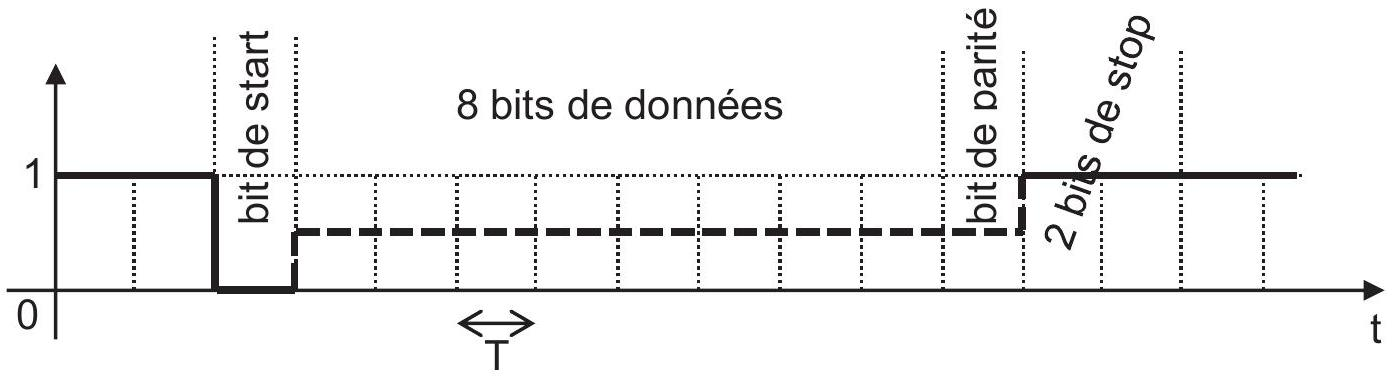
\includegraphics[max width=\textwidth, alt={}, center]{076c1ba0-5a37-41d5-876a-83fc91dd5c32-32_378_1394_1608_269}

\begin{center}
\begin{tabular}[t]{|L{0.3\textwidth}|L{0.3\textwidth}|L{0.3\textwidth}|}
\hline
\begin{tabular}[t]{L{0.9\linewidth}}
Modèle CMEN-DR v2 ©EXATECH \\
Nom de famille : \\
(Suivi, s'il y a lieu, du nom d'usage)
\includegraphics[max width=\textwidth, alt={}]{076c1ba0-5a37-41d5-876a-83fc91dd5c32-33_146_141_235_96}
 \\
\end{tabular} &  & \begin{tabular}[t]{L{0.9\linewidth}}
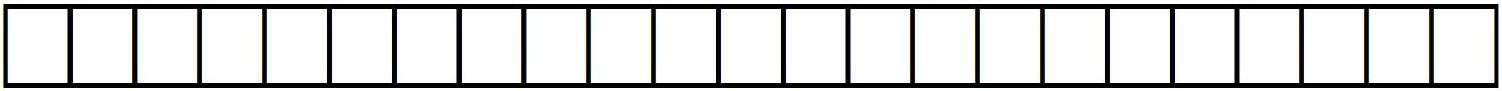
\includegraphics[max width=\textwidth, alt={}]{076c1ba0-5a37-41d5-876a-83fc91dd5c32-33_91_1502_107_470}
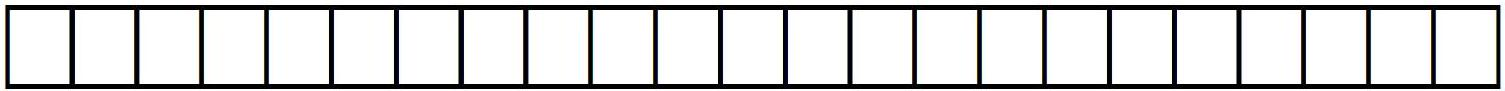
\includegraphics[max width=\textwidth, alt={}]{076c1ba0-5a37-41d5-876a-83fc91dd5c32-33_91_1505_205_468}
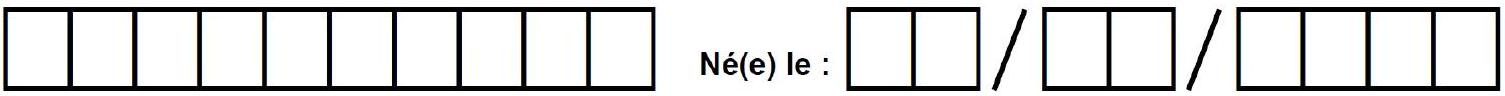
\includegraphics[max width=\textwidth, alt={}]{076c1ba0-5a37-41d5-876a-83fc91dd5c32-33_96_1505_301_470}
 \\
(Le numéro est celui qui figure sur la convocation ou la feuille d'émargement) \\
\end{tabular} \\
\hline
 &  & \begin{tabular}[t]{L{0.9\linewidth}}
(Remplir cette partie à l'aide de la notice) \\
Concours / Examen : $\_\_\_\_$ \\
Epreuve : $\_\_\_\_$ \\
\end{tabular} \\
\hline
CONSIGNES &  & \begin{itemize}[leftmargin=*, topsep=0pt, itemsep=0pt, parsep=0pt, partopsep=0pt]
  \item[-] Remplir soigneusement, sur CHAQUE feuille officielle, la zone d'identification en MAJUSCULES.
  \item[-] Ne pas signer la composition et ne pas y apporter de signe distinctif pouvant indiquer sa provenance.
  \item[-] Numéroter chaque PAGE (cadre en bas à droite de la page) et placer les feuilles dans le bon sens et dans l'ordre.
  \item[-] Rédiger avec un stylo à encre foncée (bleue ou noire) et ne pas utiliser de stylo plume à encre claire.
  \item[-] N'effectuer aucun collage ou découpage de sujets ou de feuille officielle. Ne joindre aucun brouillon.
\end{itemize} \\
\hline
\end{tabular}
\end{center}

\section*{DOCUMENTS REPONSES}
\section*{À RENDRE EN FIN D'ÉPREUVE}
Renseigner le cartouche d'identification : une feuille dont l'entête n'a pas été intégralement renseigné, ne sera pas prise en compte.

Document réponse DR1 (question 49)

\begin{figure}[h]
\begin{center}
\captionsetup{labelformat=empty}
\caption{NE RIEN ECRIRE DANS CE CADRE}
  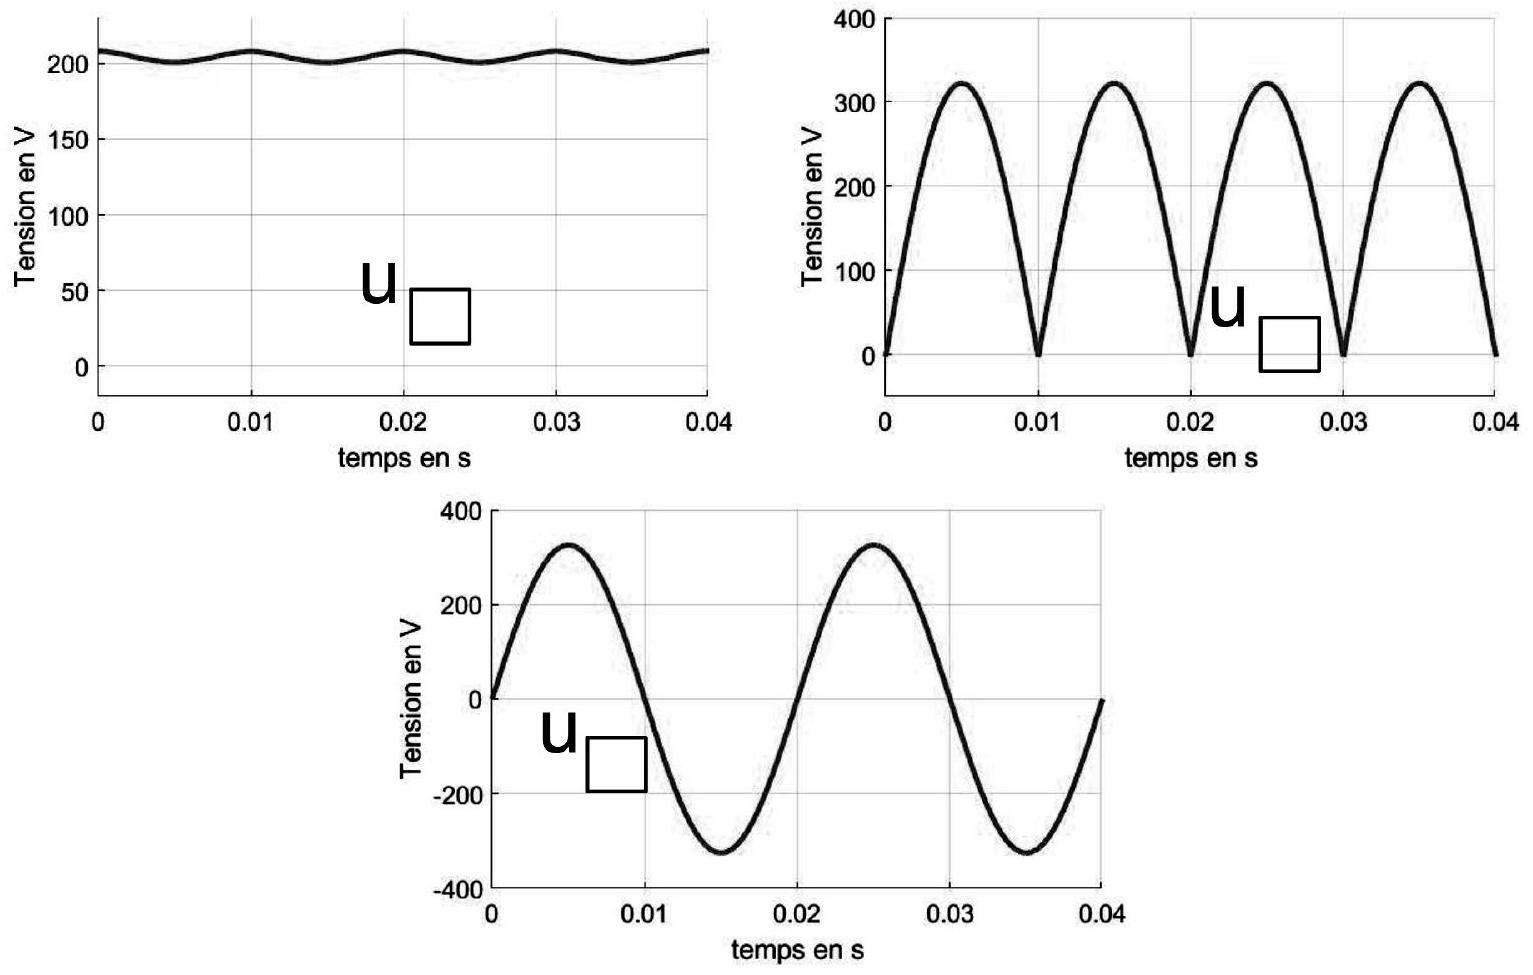
\includegraphics[alt={},max width=\textwidth]{076c1ba0-5a37-41d5-876a-83fc91dd5c32-34_975_1533_589_222}
\end{center}
\end{figure}

\section*{Document réponse DR2 (question 52)}
Loi de commande pleine onde des interrupteurs de l'onduleur. Quand $\mathrm{T}_{\mathrm{x}}$ est indiqué sur un intervalle, cela implique que l'interrupteur $\mathrm{T}_{\mathrm{x}}$ est fermé et que l'interrupteur $\mathrm{T}_{\mathrm{x}}$ ' est ouvert et vice et versa. $\omega$ est la pulsation du signal.

\begin{center}
\begin{tabular}[t]{|l|l|l|l|l|l|}
\hline
\multirow{3}{*}{} & \multicolumn{2}{|c|}{$\mathrm{T}_{1}$} & \multicolumn{2}{|c|}{$\mathrm{T}_{1}{ }^{\prime}$} &  \\
\hline
 & $\mathrm{T}_{2}{ }^{\prime}$ & \multicolumn{2}{|r|}{$\mathrm{T}_{2}$} &  &  \\
\hline
 & $\mathrm{T}_{3}$ & \multicolumn{2}{|c|}{$\mathrm{T}_{3}{ }^{\prime}$} & $\mathrm{T}_{3}$ &  \\
\hline
$\mathrm{u}_{12}$ & E &  &  &  &  \\
\hline
$\mathrm{u}_{23}$ & -E &  &  &  &  \\
\hline
$\mathrm{u}_{31}$ & 0 &  &  &  &  \\
\hline
\end{tabular}
\end{center}

\begin{center}
\begin{tabular}[t]{|l|l|l|l|l|l|l|}
\hline
\multirow{3}{*}{} & \multicolumn{2}{|c|}{$\mathrm{T}_{1}$} & \multicolumn{3}{|c|}{$\mathrm{T}_{1}{ }^{\prime}$} & \multirow{7}{*}{} \\
\hline
 & $\mathrm{T}_{2}{ }^{\prime}$ & \multicolumn{3}{|c|}{$\mathrm{T}_{2}$} & $\mathrm{T}_{2}{ }^{\prime}$ &  \\
\hline
 & $\mathrm{T}_{3}$ & \multicolumn{2}{|c|}{$\mathrm{T}_{3}{ }^{\prime}$} & \multicolumn{2}{|c|}{$\mathrm{T}_{3}$} &  \\
\hline
$\mathrm{v}_{1}$ & E/3 &  &  &  &  &  \\
\hline
$\mathrm{v}_{2}$ & -2E/3 &  &  &  &  &  \\
\hline
$\mathrm{v}_{3}$ & E/3 &  &  &  &  &  \\
\hline
\multicolumn{2}{|c|}{$0 \quad \frac{2 \pi}{6}$} & $\frac{2 \pi}{3} \quad \frac{\pi}{2}$ &  & $\frac{4 \pi}{3}$ &  &  \\
\hline
\end{tabular}
\end{center}

\begin{figure}[h]
\begin{center}
\captionsetup{labelformat=empty}
\caption{Document réponse DR3 (question 54)}
  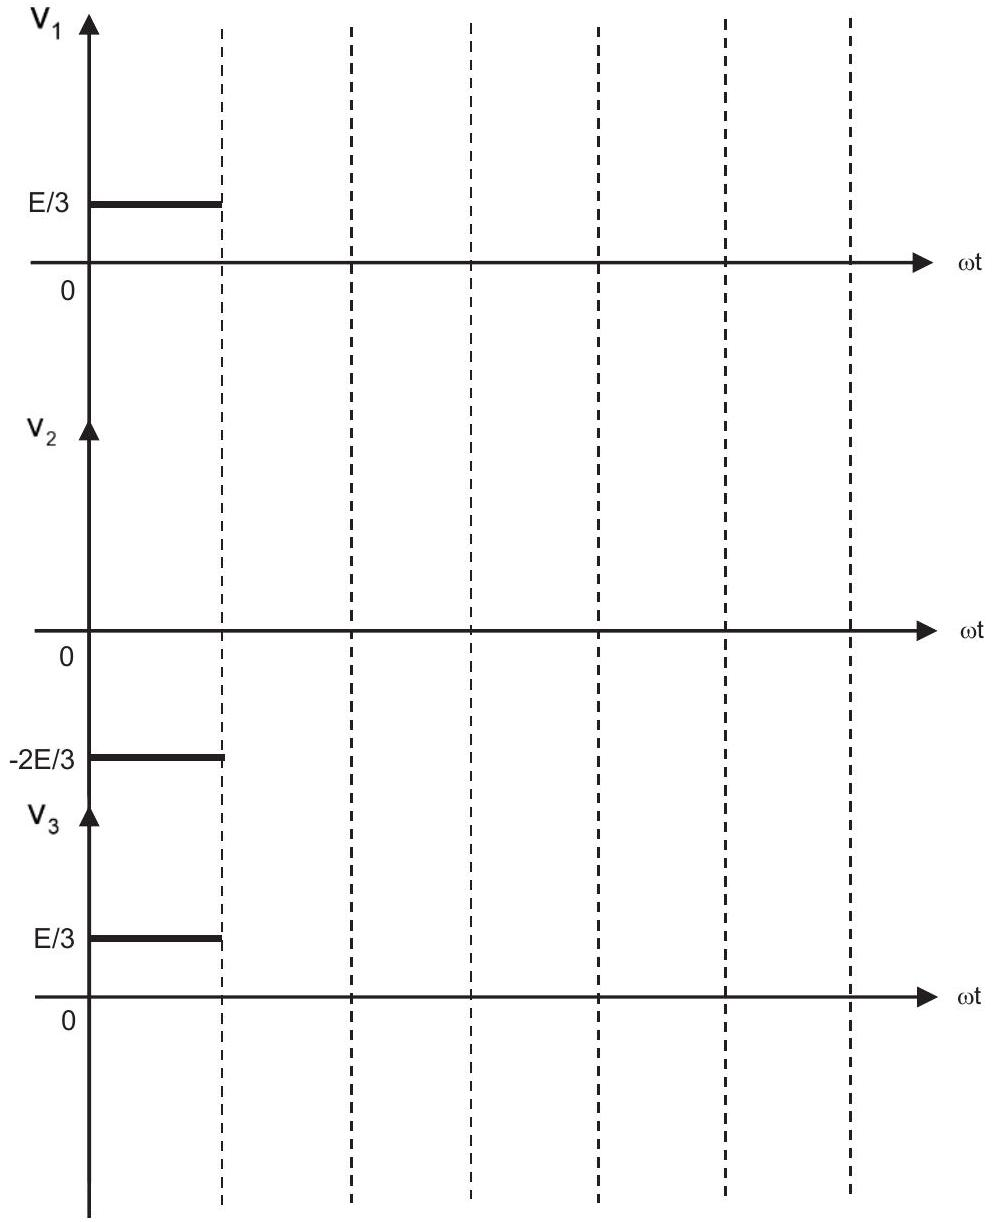
\includegraphics[alt={},max width=\textwidth]{076c1ba0-5a37-41d5-876a-83fc91dd5c32-35_1222_994_909_671}
\end{center}
\end{figure}

4 / 4


\end{document}